\documentclass[a4paper,twoside,final]{article}
%----Eingebundene Bibliotheken-----
\usepackage[ngerman]{babel}         % Deutsches Sprachpaket
\usepackage[utf8]{inputenc}         % Eingaben codieren
\usepackage[T1]{fontenc}            % Umlaute codieren, Silbentrennung
\usepackage{amsmath, amssymb}       % Mathe
\usepackage{amsthm,amstext,amsxtra} % Symbole für Mathe
\usepackage{mathtools}              % \Aboxed Boxen in align
\usepackage{wrapfig}                % Bilder umfließen
\usepackage{svg}                    % Vektorgraphiken einbinden
\usepackage{geometry}               % Papierformat
\usepackage{tabularx}               % Tabellen
\usepackage{xcolor,colortbl}        % Farben
\usepackage{graphicx}               % Für Limes Definition wichtig
\usepackage{soul}                   % Unterstreichungen
\usepackage[section]{placeins}      % \Floatbarrier
\usepackage{wrapfig}                % Bilder umfließen
\usepackage{enumerate}              % Aufzählungen
\usepackage{footnote}               % Fußzeilen
\usepackage{booktabs}               % publication quality tables
\usepackage[hyphens]{url}           % \url{}
\usepackage{bm}                     % bold symbols \bm{r}
\usepackage{dsfont}                 % identity matrix \mathds{1}
\usepackage{enumitem}               % itemize Umgebungen customizen
\usepackage{esint}                  % Doppelintegrale
\usepackage{fancyhdr}               % schöne Kopf- und Fußzeilen
\usepackage{lmodern}
\usepackage{tikz}
\usepackage{pgfmath, pgfplots}
\usepackage[labelfont=bf]{subcaption}
\usepackage[square,numbers,sort&compress]{natbib}
\usepackage{mhchem}                 % Chemistry Package
\usepackage{physics}
\usepackage{chemfig}
\usepackage[detect-all,
            locale=DE,binary-units,
            exponent-product=\cdot
            ]{siunitx}              % \SI{12}{\gram}
%siunitx stellt für Tabellen den Spaltentyp S bereit ==> Ausrichtung an Dezimaltrennzeichen
\usepackage[position=below,
            tableposition=top,
            format=hang,
            labelfont=it,
            labelfont=bf,
            ]{caption}              % Settings für Captions
\captionsetup[wrapfigure]{name=Abb.}
\usepackage[europeanvoltages,
            europeancurrents,
            europeanresistors,
            americaninductors,
            europeanports
            ]{circuitikz}           % Schaltungen
\usepackage{chngcntr}               % vor hyperref laden!
  \counterwithin*{equation}{section}
  \counterwithin*{figure}{section}
  \counterwithin*{table}{section}

\usepackage[final,
            pdfauthor={Martin Beyer, Vanessa Huth},
            pdfsubject={Fortgeschrittenen-Praktikum},
            pdffitwindow=true,      % resize document window
            pdftitle={Fortgeschrittenen-Praktikum},
            bookmarks=true,         % lesezeichen-Liste
            bookmarksopen=true,     % Lesezeichen geöffnet
            bookmarksopenlevel=1,
            bookmarksnumbered=true,
            colorlinks=true,        % fuer Druckversion auf "false"
            linkcolor=blue,         % Table of Contents, Footnotes
            urlcolor=blue,          % fuer eingebunden URLs
            citecolor=blue,         % Equations, References
            filecolor=blue,
            pdfborder={0 0 0},      % keine Rahmen um Links: {0 0 0}
            ]{hyperref}


% Commands
\renewcommand{\sfdefault}{lmss}     % latin modern sans serif
\newcommand{\R}{\mathbb{R}}         % Reelle Zahlen
\newcommand{\N}{\mathbb{N}}         % Natürliche Zahlen
\newcommand{\C}{\mathbb{C}}         % Komplexe Zahlen
\newcommand{\de}{\mathrm{d}}      % Differential
\newcommand{\entspricht}{\mathrel{\widehat{=}}}

\DeclareSIUnit{\eV}{\text{eV}}
\DeclareSIUnit{\voltpeakpeak}{\volt{\textsubscript{pp}}}

% Dokumenteneinstellungen
\setlength{\parindent}{0px}         % remove indent in new paragraph
\setlength{\parindent}{0px}         % keine Absätze durch Leerzeilen im Code
\emergencystretch=1em % Definiert den Leerraum, der innerhalb einer Zeile zusätzlich verteilt werden darf.
\setlength{\topmargin}{-5mm} % 210mm = 8.2677165in
\newlength{\mylength}
\setlength{\mylength}{\paperwidth}
\addtolength{\mylength}{-2in} % standardmäßig wird den Seitenrändern jeweils noch 1in = 25.4mm hinzuaddiert
\setlength{\textwidth}{145mm}
\setlength{\textheight}{230mm}
\addtolength{\mylength}{-\textwidth}
\setlength{\oddsidemargin}{10mm}
\addtolength{\mylength}{-\oddsidemargin}
\setlength{\evensidemargin}{\mylength}
\setlength{\marginparwidth}{1.7cm}
\interfootnotelinepenalty=10000

% Umdefinition von \textcolor ********************************************************
\makeatletter
\renewcommand*{\@textcolor}[3]{%
	\protect\leavevmode
	\begingroup
	\color#1{#2}#3%
	\endgroup
}
\makeatother
% Damit das auch im Mathemodus anwendbar ist und dort z.B. die Leerzeichen nicht wie im Textmodus gesetzt werden.

\pgfplotsset
{compat=newest, % aktuelle Version: 1.16 [29.05.2018]
	/pgf/number format/.cd, % cd steht fuer current directory
	%  	use comma, % Komma als Dezimaltrennzeichen %%% UNCOMMENT THIS !!!
	1000 sep={} % Legt das Tausendertrennzeichen fest
}
%\usepgfplotslibrary{external} % Section 7.1.1 Using the Automatic Externalization Framework of TikZ
%\tikzexternalize[prefix=FiguresTikZ/] % activate externalization! Use subdirectory [FiguresTikZ]
\usepgfplotslibrary{fillbetween}
\usepgfplotslibrary{polar}
\usetikzlibrary{arrows.meta}
\usetikzlibrary{calc}
\usetikzlibrary{datavisualization.formats.functions}
\usetikzlibrary{intersections}
\usetikzlibrary{patterns}
\usetikzlibrary{pgfplots.colormaps}
\usetikzlibrary{plotmarks}
\usetikzlibrary{shapes.geometric}

% Generelle Festlegung des Styles fuer Blockschemata (Plaene fuer Regelkreise, etc.)
\tikzstyle{block} = [draw, fill=blue!20, rectangle, minimum height=1cm, minimum width=1cm]%, minimum width=6em]
\tikzstyle{sum} = [draw, fill=blue!20, circle, node distance=1cm]
\tikzstyle{input} = [coordinate]
\tikzstyle{output} = [coordinate]
\tikzstyle{pinstyle} = [pin edge={to-,thin,black}]

\begin{document}
\setlength{\marginparsep}{2em}
\renewcommand{\theequation}{\arabic{section}.\arabic{equation}}
\renewcommand{\thefigure}{\arabic{section}.\arabic{figure}}
\renewcommand{\thetable}{\arabic{section}.\arabic{table}}

% Anfang ********************************************************
\begin{center}
\thispagestyle{empty}
  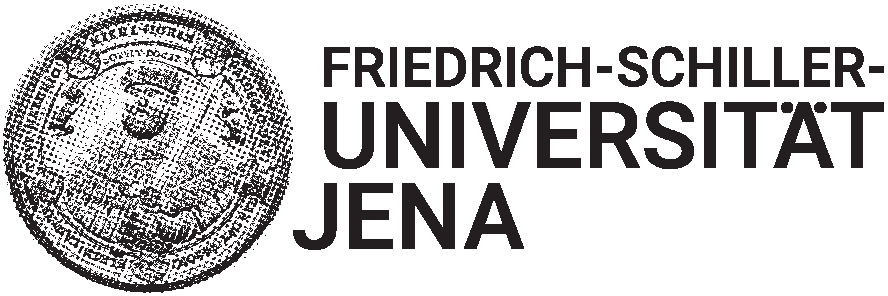
\includegraphics[width=0.75\textwidth]{../UniJena_BildWortMarke_black.pdf}\\[4em]
  \Large
  Ausarbeitung zum Versuch\\[2em]
  \Huge
  Mößbauer Spektroskopie\\
  \vspace{2cm}
  \Large
  Martin Beyer und Vanessa Huth\\[2em]
  Abgabe: 14. Januar 2020\\[2em]
  Betreuer: Dr. Udo Reislöhner\\[5em]
  \begin{flushleft}
  	Bewertung und Ausarbeitung:\\[2em]
		Protokollführung und Form:\\[1em]
		Ergebnisse, Auswertung und Interpretation:\\[1em]
		Bemerkungen und Hinweise des Betreuers:
  \end{flushleft}
\end{center}
\clearpage

\pagestyle{fancy}
\renewcommand{\headrulewidth}{0pt}
\renewcommand{\footrulewidth}{0.5pt}
\renewcommand{\sectionmark}[1]{\markright{#1}}
\fancyhead[RO,LE]{\textbf{Mößbauer Spektroskopie}}
\fancyhead[RE,LO]{\rightmark}
\fancyfoot[LE,RO]{\bfseries\thepage}
\fancyfoot[CO,CE]{Protokoll}
\renewcommand{\headrulewidth}{0.5pt}
\renewcommand{\footrulewidth}{0.5pt}

\setcounter{equation}{0}
\setcounter{figure}{0}

% *********************************************
% ***** KAPITEL 1 *****************************
% *********************************************
\tableofcontents
% \pagenumbering{gobble}% remove page numbering
\newpage
% \pagenumbering{arabic}
\section{Aufgabenstellung} \label{sec:Aufgabenstellung}
\subsection{Abschätzung einer oberen Strahlendosis}
\paragraph{Aufgabe 1}$~$\\
Abschätzung der oberen Grenze der zusätzlichen Äquivalenzdosis einer $^{60}$Co-Quelle die ohne Abschirmung 12 Stunden lang in einem Meter Abstand steht. Das Ergebnis wird mit der durchschnittlichen Strahlenbelastung eines Bürgers verglichen.
\subsection{Messung des Energiespektrums der $^{57}$Co-Quelle}

\paragraph{Aufgabe 2a}$~$\\
Es wird das Energiespektrum der $^{57}$Co-Quelle aufgenommen, mit dem Oszilloskop das Ausgangssignal des Verstärkers gemessen und der Zusammenhang mit dem Energiespektrum hergestellt. Die Verstärkung wird variiert.
\paragraph{Aufgabe 2b}$~$\\
Mithilfe verschiedener Strahler wird eine Energiekalibrierung durchgeführt und die \SI{14,4}{\kilo\text{e}\volt}-Linie identifiziert.

\subsection{Einstellung des Energiefensters auf die \SI{14,4}{\kilo\text{e}\volt}-Linie}
\paragraph{Aufgabe 3a}$~$\\
Das Fenster des Einkanal-Diskriminators wird auf die Resonanzabsorptionslinie eingestellt, indem das Energiesignal mit dem Ausgangssignal des \textit{SCA} (\textit{Single channel Scaling}) getriggert wird.
\paragraph{Aufgabe 3b}$~$\\
Mithilfe des Vielkanalanalysators wird durch die Triggerung des ADC über den Gate-Eingang kann die Wirkung der Fenstereinstellung am \textit{SCA} direkt am Vielkanalanalysator beobachtet werden. Gegebenenfalls wird die Fenstereinstellung nachjustiert und der eingestellte Bereich im Energiespektrum skizziert.

\subsection{Messung und Auswertung von Mößbauerspektren}
\paragraph{Aufgabe 4a}$~$\\
Das Mößbauerspektrum von natürlichem Eisen wird gemessen und erklärt.
Dabei wird folgendes bestimmt:
\begin{itemize}
  \item Energieaufspaltung $\Delta E_g$ im Grundzustand und $\Delta E_a$ im angeregten Zustand und Vergleich mit der Energie der $\gamma$-Quanten
  \item Betrag des $B$-Feldes am Ort der $^{57}$Fe-Kerne
  \item das magnetische Moment des ersten angeregten Zustands
  \item die Isomerieverschiebung bezüglich der Quelle
  \item die Linienbreite für große und kleine Geschwindigkeiten
\end{itemize}
\paragraph{Aufgabe 4b}$~$\\
Das Mößbauerspektrum von Edelstahl wird gemessen und disktutiert (Linienzahl, Isomerieverschiebung, Linienbreite).
\paragraph{Aufgabe 4c}$~$\\
Das Mößbauerspektrum von Eisensulfat wird gemessen und diskutiert (Linienzahl, Energieaufspaltung, Isomerieverschiebung, Linienbreite).
% *********************************************
% ***** KAPITEL 2 *****************************
% *********************************************
\newpage
\section{Grundlagen} \label{sec:Grundlagen}
\subsection{Mößbauerspektroskopie}

\subsubsection{Der $\gamma$-Zerfall des Kerns und Rückstoßenergieverlust}\label{sec:Rückstoss}
Atomkerne besitzen diskrete Energieniveaus. Beim Übergang von einem höheren zu einem niedrigeren Energieniveau kommt es häufig zur Emission von $\gamma$-Strahlung. Dabei gilt Energie-, Drehimpuls- und Praitätserhaltung. Wird ein $\gamma$-Quant emittiert, wird dem emittierenden Kern dabei ein Rückstoß erteilt. So erhält das Quant nicht die gesamte Anregungsenergie. \\
Für ein einatomiges Gas im thermischen Gleichgewicht gilt für die Energie des angeregten Atomkerns vor der Emission:
\begin{align}
E_\text{vor} = E_a+\frac{\vec{p}^2}{2M},
\end{align}
wobei $\vec{p} = M\vec{v}$ der Impuls und $M$ die Masse des Atoms ist. \\
Der Impuls ist aufgrund der Impulserhaltung nach der Emission um den Impuls des $\gamma$-Quants $\hbar\vec{k}$ reduziert. Außerdem muss hier die Energie im Grundzustand $E_g$ verwendet werden. Nach der Emission beläuft sich die Energie des Atomkerns also auf
\begin{align}
E_\text{nach} = E_g+\frac{(\vec{p}-\hbar\vec{k})^2}{2M}.
\end{align}
Somit ergibt sich die Energiedifferenz und damit die Energie des emittierten Quants zu:
\begin{align}\label{equ:EnergieGamma}
E_\text{vor}-E_\text{nach}= \hbar \omega = \hbar \omega_0 + \hbar (\vec{k}\cdot\vec{v})-\frac{\hbar^2\vec{k}^2}{2M}.
\end{align}

\subsubsection{Natürliche Linienbreite}
Aufgrund der Unschärferelation muss es eine Energieunschärfe der $\gamma$-Quanten geben. Bei genauerer Betrachtung wird ersichtlich, dass das Frequenzspektrum der emittierten $\gamma$-Strahlung eine Lorentz-Verteilung um die Freqenz $\omega_0$ mit der Halbwertsbreite $\frac{\Gamma}{\hbar}$ ist. Es gilt
\begin{align}
I(\omega) = \frac{I_0}{1+[(\omega-\omega_0)2\hbar/\Gamma]^2}
\end{align}
wobei I($\omega$) die Intensität der Strahlung mit der Frquenz $\omega$ angibt.
$\Gamma$ ist die sogenannte natürliche Linienbreite und gibt die Energieunschärfe an. Für sie gilt:
\begin{align}
\Gamma = \hbar / \tau_N
\end{align}
mit $\tau_N$ der mittleren Lebensdauer des Kernzustands.

\subsubsection{Der Mößbauereffekt}
Ein $\gamma$-Quant kann beim Auftreffen auf einen Atomkern nur absorbiert werden, wenn die Energie des Quants gerade der Anregungsenergie eines Kernniveaus entspricht. \\
Der naheliegende Gedanke, dies sei immer gegeben, wenn Emission und Absorption am gleichen Kernübergang erfolgen, ist aufgrund des in \ref{sec:Rückstoss} beschriebenen Effekts jedoch falsch. Außerdem wird beim Absorbieren aus Impulserhaltungsgründen ein Teil der Energie des Quants in kinetische Energie des Kerns umgewandelt. \\
Ein $\gamma$-Quant kann also bei der Verwendung von Atomen der gleichen Sorte zur Emission und Absorption nur absorbiert werden, wenn beide Vorgänge unverschoben erfolgen, also beidenfalls eine Energieverschiebung vermieden wird. Dies kann durch den Einbau der Atome in ein Kristallgitter gewährleistet werden. In diesem Fall wird bei einem Teil der Emissionen der Rückstoß auf den gesamten Kristall übertragen, womit aufgrund dessen viel größerer Masse praktisch keine Energieübertragung verbunden ist. Dann gilt unter Verwendung von \eqref{equ:EnergieGamma}
\begin{align}\label{eqn:Dopplereffekt}
\hbar\omega = \lim\limits_{M \to \infty}{\left(\hbar \omega_0 + \hbar (\vec{k}\cdot\vec{v})-\frac{\hbar^2\vec{k}^2}{2M}\right)} = \hbar\omega_0+\hbar(\vec{k}\vec{v}).
\end{align}

\subsubsection{Mößbauer-Apparatur}
Der prinzipielle Aufbau der Mößbauer-Apparatur ist in Abbildung \ref{fig:Apparatur} dargestellt. Die grundsätzlichen Bestandteile der Apperatur sind die radioaktive Quelle, welche bewegt werden kann, ein Absorber und ein Detektor. Es werden zwei unterschiedliche Aufbauarten unterschieden: die Transmissionsgeometrie, in welcher ein Minimum des Signals bei der Geschwindigkeit wo Resonanzabsorption auftritt, festgestellt wird und eine Streugeometrie, bei welcher die Floureszensstrahlung nachgewiesen wird.
\begin{figure}[htp]
    \centering
    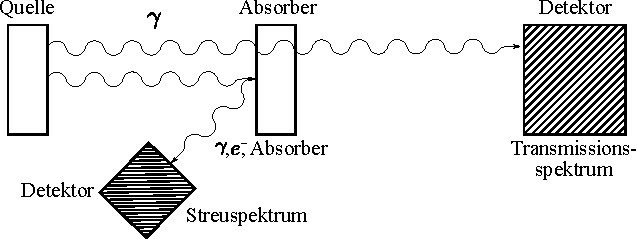
\includegraphics[width=0.7\textwidth]{Bilder/Apparatur.pdf}
    \caption{Aufbau der Mößbauer-Apparatur nach \cite{Schatz} S.58 (eigene Abbildung).}
    \label{fig:Apparatur}
\end{figure}

\subsubsection{Debye-Waller-Faktor}
Der \textsc{Debye}-\textsc{Waller}-Faktor (DWF) ist der Anteil der unverschobenen $\gamma$-Emissionen zu allen $\gamma$-Emissionen. Er lässt sich auf
\begin{align}
f(T) = \exp\left(-\frac{\hbar k^2}{6MN}\int_{0}^{\infty} \frac{Z(\Omega)}{\Omega}\left[1+\frac{2}{\exp(\frac{\hbar\Omega}{k_B T}-1)}\right] d\Omega\right)
\end{align}
bestimmen, wobei $Z(\Omega)$ die Phononenzustandsdichte beschreibt. Für tiefe Temperaturen im Rahmen des \textsc{Debye}-Modells ergibt sich
\begin{align}\label{eqn:Debye-Waller}
f_D(T) = \exp\left(-\frac{\hbar^2k^2}{2M}\frac{3}{2k_B\Theta}\left[1+\frac{2\pi^2}{3}\left(\frac{T}{\Theta}\right)^2\right]\right).
\end{align}
Der DWF ist temperaturabhängig und zeigt ein Maximum bei T = 0. Auch beim absoluten Nullpunkt gilt $f < 1$ aufgrund der Nullpunktschwingung. Allgemein sollte die Temperatur nicht zu groß werden und die \textsc{Debye}-Temperatur $\Theta$ nicht überschreiten.\\
Mit wachsender Rückstoßenergie $\hbar^2k^2/2M$ wird der DWF kleiner. Aufgrund des Zusammenhangs $\hbar k = E_\gamma / c $, bedeutet das direkt, dass auch für größere $E_\gamma$ der DWF kleiner wird. Um also einen für den Mößbauereffekt bedeutsamen großen \textsc{Debye}-\textsc{Waller}-Faktor zu erhalten, ist es wichtig, dass die $\gamma$-Energie nicht zu groß wird.

\subsubsection{Mößbauerquellen}
Da die Absoprtion im Allgemeinen nur durch einen Kern im Grundzustand erfolgen wird, können nur Emissionsübergänge, die zum Grundzustand führen verwendet werden. Der \textsc{Debye}-\textsc{Waller}-Faktor des als Quelle verwendeten Stoffes darf nicht zu klein sein. Aufgrund von \eqref{eqn:Debye-Waller} sind dafür eine nicht zu große $\gamma$-Energie, hohe \textsc{Debye}-Temperatur und große Atommasse günstig. Um eine nicht zu große Linienbreite zu erhalten und damit eine zu schlechte Energieauflösung zu vermeiden, darf die Lebensdauer des entsprechenden Mößbauerniveaus nicht zu kurz sein. Außerdem sollten die Eigenschaften des Mutterisotops (Lebensdauer, chemische und metallurgische Eigenschaften usw.) und die Herstellungsmöglichkeiten des Isotops günstig sein.


\paragraph{Zerfallsschema \textsuperscript{57}Co}
In Abbildung \ref{fig:Zerfallsschema} ist das Zerfallsschema von \textsuperscript{57}Co dargestellt. \textsuperscript{57}Co zerfällt überwiegend über den Einfang eines Elektrons aus der K-Schale der Atomhülle in den angeregten Zustand I = 3/2 des \textsuperscript{57}Fe. Dabei entsteht ein Loch in der K-Schale, welches durch ein Elektron aus einer höheren Schale unter Emission von \SI{6,4}{\keV} Röntgenstrahlung wieder aufgefüllt wird. Das angeregte \textsuperscript{57}Fe geht dann unter $\gamma$-Emission bzw. innerer Konversion in den Grundzustand I = 1/2 über.\\
Das im Versuch verwendete \textsuperscript{57}Co - \textsuperscript{57}Fe eignet sich aufgrund mehrerer Eigenschaften als Mößbauerquelle: Mit 270 Tagen ist die Halbwertszeit des Mutterisotops ausreichend lang um ein zu häufiges Wechseln zu vermeiden, die Lebensdauer des Mößbauerniveaus von $t_{1/2}=\SI{98}{\nano\second}$ ermöglicht eine ausreichende Energieauflösung und die Energie von \SI{14,4}{\electronvolt} ist hinreichend klein, um auch bei Zimmertemperatur einen hohen \textsc{Debye}-\textsc{Waller}-Faktor zu gewährleisten.
\begin{figure}[htp]
    \centering
    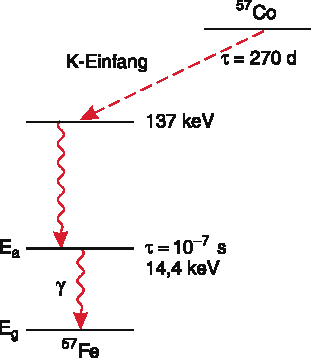
\includegraphics[width=0.3\textwidth]{Bilder/Zerfallsschema_Kobalt.pdf}
    \caption{Zerfallsschema \textsubscript{57}Co aus \cite{Demtroeder} S. 416}
    \label{fig:Zerfallsschema}
\end{figure}


\subsubsection{Hyperfeinwechselwirkung}
Hyperfeinwechselwirkung ist die Wechselwirkung des Kerns mit elektrischen oder magnetischen Feldern, die im Festkörper von Elektronen oder Atomrümpfen in der Umgebung des Kerns hervorgerufen oder auch extern angelegt werden.
\paragraph{Magnetische Wechselwirkung}
Bei magnetischer Wechselwirkung ergibt sich eine Wechselwirkungsenergie bzw. Zusatzenergie
\begin{align}\label{equ:Emag}
E_\text{magn} = - \vec{\mu}\cdot\vec{B},
\end{align}
wobei $\vec{\mu}$ das magnetische Kerndipolmoment und $\vec{B}$ die magnetische Flussdichte am Kernort ist, die zu einer zeitlichen Veränderung des Kernspins und  der Aufhebung der energetischen M-Entartung der Kerniveaus führt:\\
Aufgrund von \eqref{equ:Emag} hängt $E_\text{magn}$ vom Winkel zwischen $\vec{B}$ und $\vec{\mu}$ ab. Wegen der quantenmechanischen Richtungsquantelung des Drehimpulses und sich damit ergebenden bestimmten Einstellungsmöglichkeiten von $\vec{\mu}$, folgt eine äquidistante Aufspaltung zwischen benachbarten M-Zuständen. Denn es gilt (wenn die $z$-Achse parallel zum $\vec{B}$-Feld)
\begin{align}
E_\text{magn} &= -\gamma B \hbar M\\
              &= - \frac{\mu}{I} B M \qquad \text{mit} \quad \gamma = \dfrac{\mu}{\hbar I}.
\end{align}
Die Aufspaltung von angeregtem und Grundzustand ergibt sich nun zu
\begin{align}\label{eqn:Magnetfeld}
  \Delta E = - \frac{\mu}{I} B,
\end{align}
da zwischen benachbarten Zuständen $\Delta M = 1$ gilt.
Für \textsuperscript{57}Fe können experimentell die sechs für M1-Strahlung erlaubten Übergänge (siehe dazu das Termschema von Eisen in Abbildung~\ref{fig:Termschema_Eisen} auf Seite~\pageref{fig:Termschema_Eisen}) zwischen Grundzustand und angeregtem Zustand beobachtet werden. Für die Übergangsenergien gilt:
\begin{align}
\hbar\omega (M_a \rightarrow M_g) = \left(E_a - \frac{\mu_a} {I_a} M_a B \right) - \left(E_g - \frac{\mu_g} {I_g} M_g B \right)  = \hbar\omega_0 - \left(\frac{\mu_a }{I_a} M_a - \frac{\mu_g}{I_g} M_g\right) B.
\end{align}

\paragraph{Linienintensität} Je nach Magnetisierung der untersuchten Probe ergibt sich eine unterschiedliche Intensität der beobachteten Mößbauerlinien. Bei einer statistischen Verteilung des $\vec{B}$-Feldes lässt sich für eine unmagnetisierte Probe ein Intensitätsverhältnis von $1:2:3$ beobachten.\\
Liegt jedoch eine Korrelation zwischen $\vec{B}$-Feld und Ausbreitungsrichtung des $\gamma$-Quants vor, dann ändern sich die Linienintensitäten und es ergeben sich zwei Spezialfälle:
\begin{enumerate}
  \item $\vec{B}$-Feld parallel zur Ausbreitungsrichtung: Die Linien für $M=0$ sind nicht beobachtbar und das Intensitätsverhältnis lautet $1:0:3$.
  \item $\vec{B}$-Feld senkrecht zur Ausbreitungsrichtung: Es ergibt sich ein Verhältnis von $1:4:3$.
\end{enumerate}

\subsubsection{Isomerieverschiebung}
Aufgrund der elektrostatischen Wechselwirkung des ausgedehnten Kerns mit den Elektronen am Kernort ergibt sich eine Energieverschiebung zwischen der Energie eines Kernzustandes für einen ausgedehnten Kern und der Energie des Kernzustands für einen punktförmigen Kern.
Bei der Mößbauerspektroskopie wird diese Energiedifferenz durch die Bewegung der Quelle $Q$ relativ zum Absorber $A$ unter Nutzung des Dopplereffekts ausgeglichen. Als Isomerieverschiebung $v_\text{res}$ wird hier die Geschwindigkeit der Quelle, bei der Resonanzabsorption auftritt, bezeichnet (wenn Hyperfeinstrukturwechselwirkungen vernachlässtigt werden können)
\begin{align}
  v_\text{res} = \frac{Z e^2 c}{6\varepsilon_0 \hbar \omega_0}(|\Psi_A(0)|^2-|\Psi_Q(0)|^2)(<r_a^2>-<r_g^2>),
\end{align}
wobei $\Psi$ die Wellenfunktion der Elektronen am Kernort bezeichnet und $<r^2>$ den mittlere quadratische Kernradius ist.
Die Isomerieverschiebung tritt nur dann auf, wenn
\begin{align}
  |\Psi_A(0)|^2-|\Psi_Q(0)|^2 \neq 0 \quad \text{und} \quad <r_a^2>-<r_g^2> \neq 0.
\end{align}
Für $^{57}$Fe ist die Größe $<r_a^2>-<r_g^2>$ negativ, der angeregte Zustand besitzt einen kleineren Kernradius als der Grundzustand.
Bei Vorliegen einer Aufspaltung wird im Mößbauerspektrum als Isomerieverschiebung die Abweichung des Schwerpunkts zweier zueinandergehörender Minima von der Null bezeichnet.

\subsubsection{Elektrische Quadropulaufspaltung}
Wenn der deformierte Kern mit einem elektrischen Feldgradienten wechselwirkt, kommt es zur Aufhebung der Energieentartung bezüglich der $M$-Unterzustände. Die zugehörige Energiedifferenz wird durch die Geschwindigkeitsdifferenz der sich ergebenden Minima bestimmt.

\subsection{Nachweis von $\gamma$-Strahlung}
Bei der Wechselwirkung von $\gamma$-Strahlung mit der Materie werden drei Prozesse beobachtet: Paarbildung, Comptoneffekt und Photoeffekt. Zum Nachweis von $\gamma$-Strahlung werden die zwei letzteren grundlegenden Prozesse verwendet.
\subsubsection{Photoeffekt}
Beim Photoeffekt überträgt das $\gamma$-Quant seine komplette Energie auf ein \textit{gebundenes} Elektron. Für die Energie des Elektrons gilt $E_e = E_\gamma - E_B$. Auch die Bindungsenergie steht für den Szintillationsprozess zur Verfügung. Zunächst als Anregungenergie im Atom zurückbleibend wird sie unmittelbar über Auger-Elektronen oder Röntgenstrahlung frei. Es ergibt näherungsweise folgende Proportionalität:
\begin{align}
\sigma  \propto E_{\gamma} ^{-7/2} Z^5.
\end{align}
\subsubsection{Comptoneffekt}
Der Compton-Effekt ist die elastische Streuung eines $\gamma$-Quants an \textit{freien} Elektronen. Von quasifreier Streuung wird gesprochen, wenn die Elektronen im Atom gebunden sind, die Bindungsenergie aber bei den äußeren Elektronen vernachlässigt werden kann. Die Energie des Photons ändert sich, die Wellenlänge wird größer, das gestoßene Elektron wird frei und seine Energie ist abhängig vom Streuwinkel. Hierbei gilt folgende Proportionalität:
\begin{align}
\sigma \propto E_{\gamma}^{-1} Z.
\end{align}
\subsubsection{Szintillationsdetektor}
Zum eigentlichen Nachweis werden die durch Photo- oder Comptoneffekt freigesetzten Elektronen verwendet. Hierzu wird z.\,B. ein Szintillationsdetektor verwendet, dessen Aufbau in Abbildung \ref{fig:Szintillationsdetektor} ersichtlich wird.\\
Der $\gamma$-Quant trifft auf den Szintillator und erzeugt durch Photo- und Comptoneffekt Primärelektronen. Das Primärelektron wird abgebremst und ionsiert die Szinitllatoratome (oder regt sie an). Dabei ist die Anzahl der ionisierten Atome proprtional zur Energie des Elektrons. Es kommt zu einer Rekombination dieser unter Aussendung von Licht. Dieses Licht löst dann aus der Photokathode Elektronen aus, welche an den Dynoden des Primärelektronenvervielfachers verstärkt werden.
\begin{figure}[htp]
    \centering
    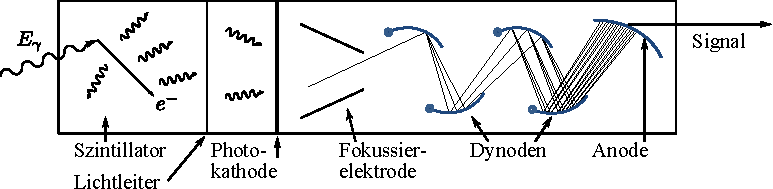
\includegraphics{Bilder/Szintillationsdetektor.pdf}
    \caption{Prinzipskizze eines Szintillationsdetektors nach \cite{Schatz} S.28 (eigene Abbildung).}
    \label{fig:Szintillationsdetektor}
\end{figure}

\subsection{$\gamma$-Spektrum}
Das Spektrum von \textsuperscript{137}Cs ist beispielhaft in Abbildung \ref{fig:CsSpek} dargestellt. An diesem werden die charakteristischen Elemente eines $\gamma$-Spektrums im Folgenden erklärt.
\begin{figure}[htp]
    \centering
    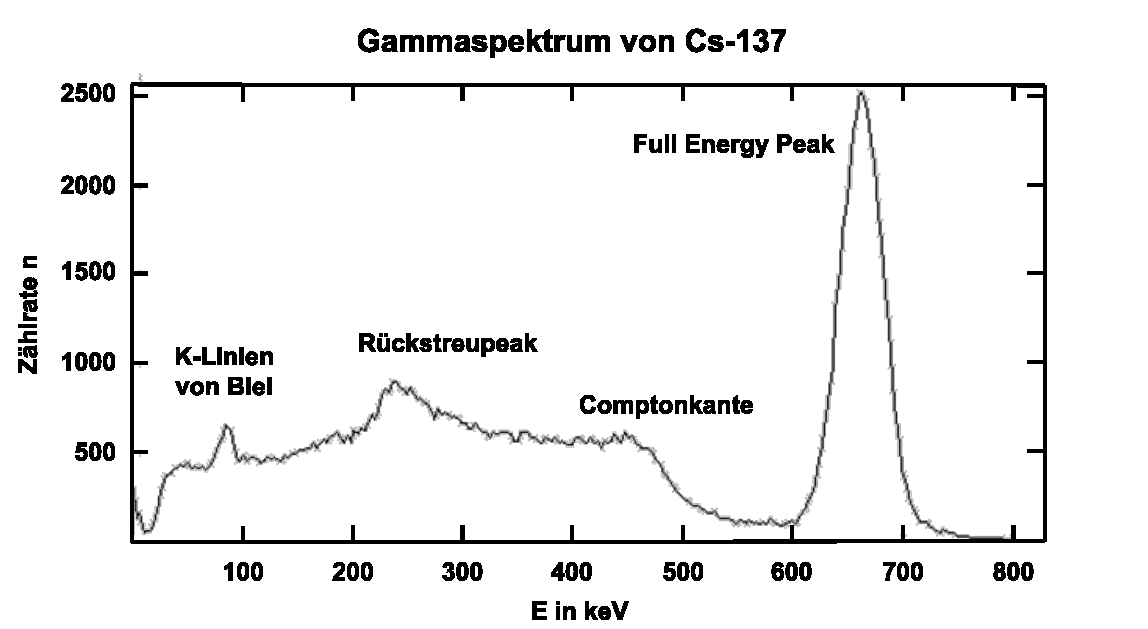
\includegraphics[width=0.7\textwidth]{Bilder/gamma-spektrum-cs137.pdf}
    \caption{$\gamma$-Spektrum von \textsuperscript{137}Cs aus \cite{Leifi}.}
    \label{fig:CsSpek}
\end{figure}\\
Bei \SI{662}{\kilo\electronvolt} befindet sich die \textit{Gesamtabsoptionslinie}, auch Photopeak genannt. Bei dieser Energie tritt der Photoeffekt auf, das Photon gibt seine gesamte Energie an ein gebundenes Elektron ab. Da die Anzahl der ionisierten Atome von der Energie des Elektrons abhängt, ist hier ein deutliches Peak zu erkennen. Das \textit{Comptonkontinuum} bezeichnet die über einen breiten Energiebereich verteilten Ereignisse im niederenergetischen Bereich des Spektrums. Für das Auslösen der Elektronen ist in diesem Bereich hauptsächlich der Comptoneffekt verantwortlich. Dabei wird nur ein Teil der Energie des $\gamma$-Quants an die Elektronen abgegeben. Außerdem ist die Energie der freiwerdenden Elektronen abhängig vom Streuwinkel und damit kontinuierlich. Für \SI{180}{\degree} wird ein maximaler Energiebetrag erreicht. Dieser markiert die \textit{Comptonkante}. Die \textit{Rückstreulinie} ergibt sich, da das radiaktove Präparat in alle Richtungen emittiert. So kommt es vor, dass Quanten in die dem Zähler entgegengesetzte Richtung gestrahlt werden in der Nähe des Präparats Compton gestreut werden und als Streuquanten vom Szintillationsdetektor registriert werden. Wird den Zusammenhang zwischen Streuwinkel und Energie des gestreuten Quants genauer, kann festgestellt werden, dass Energiequanten im Winkelbereich zwischen \SI{100}{\degree} und \SI{180}{\degree} einem eng begrenzten Energiebereich zugeordnet werden. Diese Quanten werden mittels Photoeffekt im Szintillationskristall registriert, weshalb sich ein Maximum ergibt. Außerdem erscheint im Spektrum die $K$-Röntgen-Linie von Blei, da eine Bleiabschirmung verwendet wurde.
% *********************************************
% ***** KAPITEL 3 *****************************
% *********************************************
\section{Messapparatur und Versuchsdurchführung} \label{sec:Versuchsdurchführung}
\subsection{Messung des Energiespektrums der \textsuperscript{57}Co-Quelle}
\begin{figure}[htp]
    \centering
    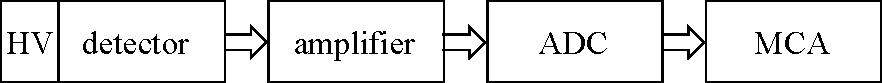
\includegraphics[width=0.8\textwidth]{Schaltungen/Blockschaltbild_Energiespektren.pdf}
    \caption{Blockschaltbild zur Messung von Energiespektren nach \cite{Reisloehner} (eigene Abbildung).}
    \label{fig:BlockEnergiespektren}
\end{figure}
Zur Messung des Energiespektrums wird nach dem in Abbildung \ref{fig:BlockEnergiespektren} gezeigten Schema vorgegangen: Die $\gamma$-Strahlung wird mit einem NaI(TI)-Szintillationsdetektor registriert, das Detektorsignal wird anschließend verstärkt (amplifier), digitalisiert (Analog-Digital-Converter) und in einem der jeweiligen Impulshöhe entsprechenden Kanal eines Histogrammspeichers (Multi-Channel-Analyser) abgelegt, sodass die Zahl der Ereignisse über der jeweils im Detektor deponierten Energie dargestellt wird. Dieses Verfahren wird Puls-Höhen-Analyse genannt (PHA). \\
Das Ausgangssignal des Verstäkers wird zusätzlich am Ozilloskop dargestellt, um den Zusammenhang zwischen Energiespektrum und Ausgangssignal des Verstärkers herzustellen.
\paragraph{Energiekalibrierung}
Um den einheitenlosen Kanälen eine Energie zuzuordnen werden \textsuperscript{133}Ba und \textsuperscript{241}Am zur Kalibrierung verwendet. Beide Stoffe werden in die Absorberhalterung eingesetzt und deren charakteristische Linien im Spektrum identifiziert. Dadurch wird eine Kalibrierung der Achse vorgenommen und die \SI{14,4}{\kilo\electronvolt} Linie des \textsuperscript{57}Co kann bei Aufnahme der Spektren identifziert werden.
\newpage
\subsection{Einstellung des Energiefensters auf die \SI{14,4}{\kilo\electronvolt} Linie}\label{sec:Energiefenster}
\paragraph{Einstellung mit dem Oszilloskop}
Das Fenster des Einkanal-Diskriminators wird auf die Resonanzabsoprtionslinie bei \SI{14,4}{\kilo\electronvolt} eingestellt, indem das Energiesignal mit dem Ausgangssignal des \textit{SCA} getriggert wird. \\
Dazu wird der Ausgang des Amplifiers (Energiesignal) an den Eingang des \textit{SCA}
%haben wir das gemacht???%
und an den Oszilloskop-Eingang 1 angelegt und der Ausgang des \textit{SCA} mit dem Oszilloskop-Eingang 2 verbunden. Das entstehende Bild zeigt Abbildung~\ref{fig:Oszilloskop}.
\begin{figure}[htp]
    \centering
    \begin{subfigure}{0.45\textwidth}
        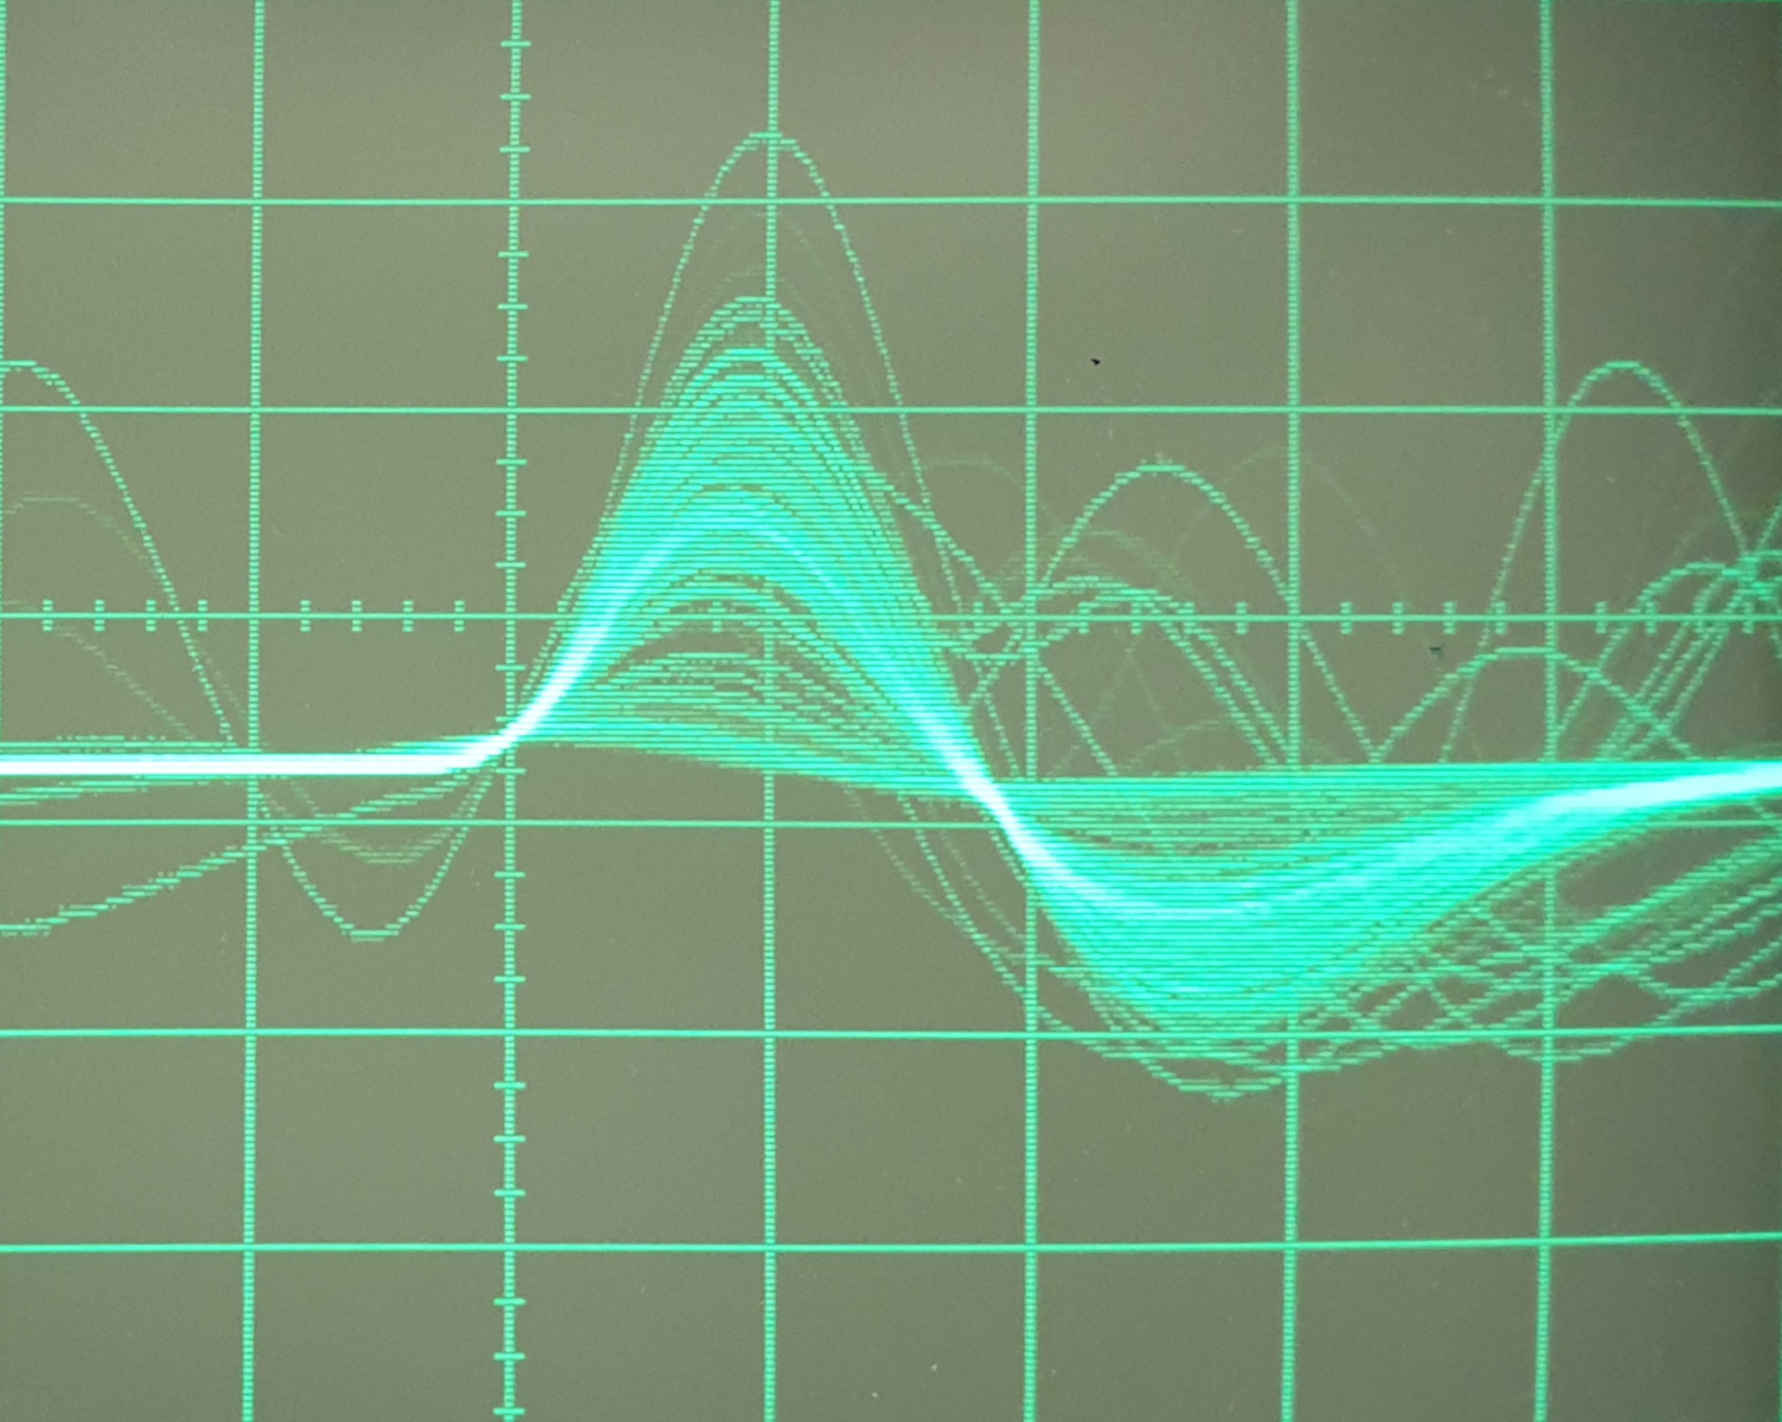
\includegraphics[width=\textwidth]{Bilder/1209_151002.jpg}
        \caption{Darstellung der Energiesignale am Oszilloskop.}
    \end{subfigure}
    \hspace{1cm}
    \begin{subfigure}{0.45\textwidth}
        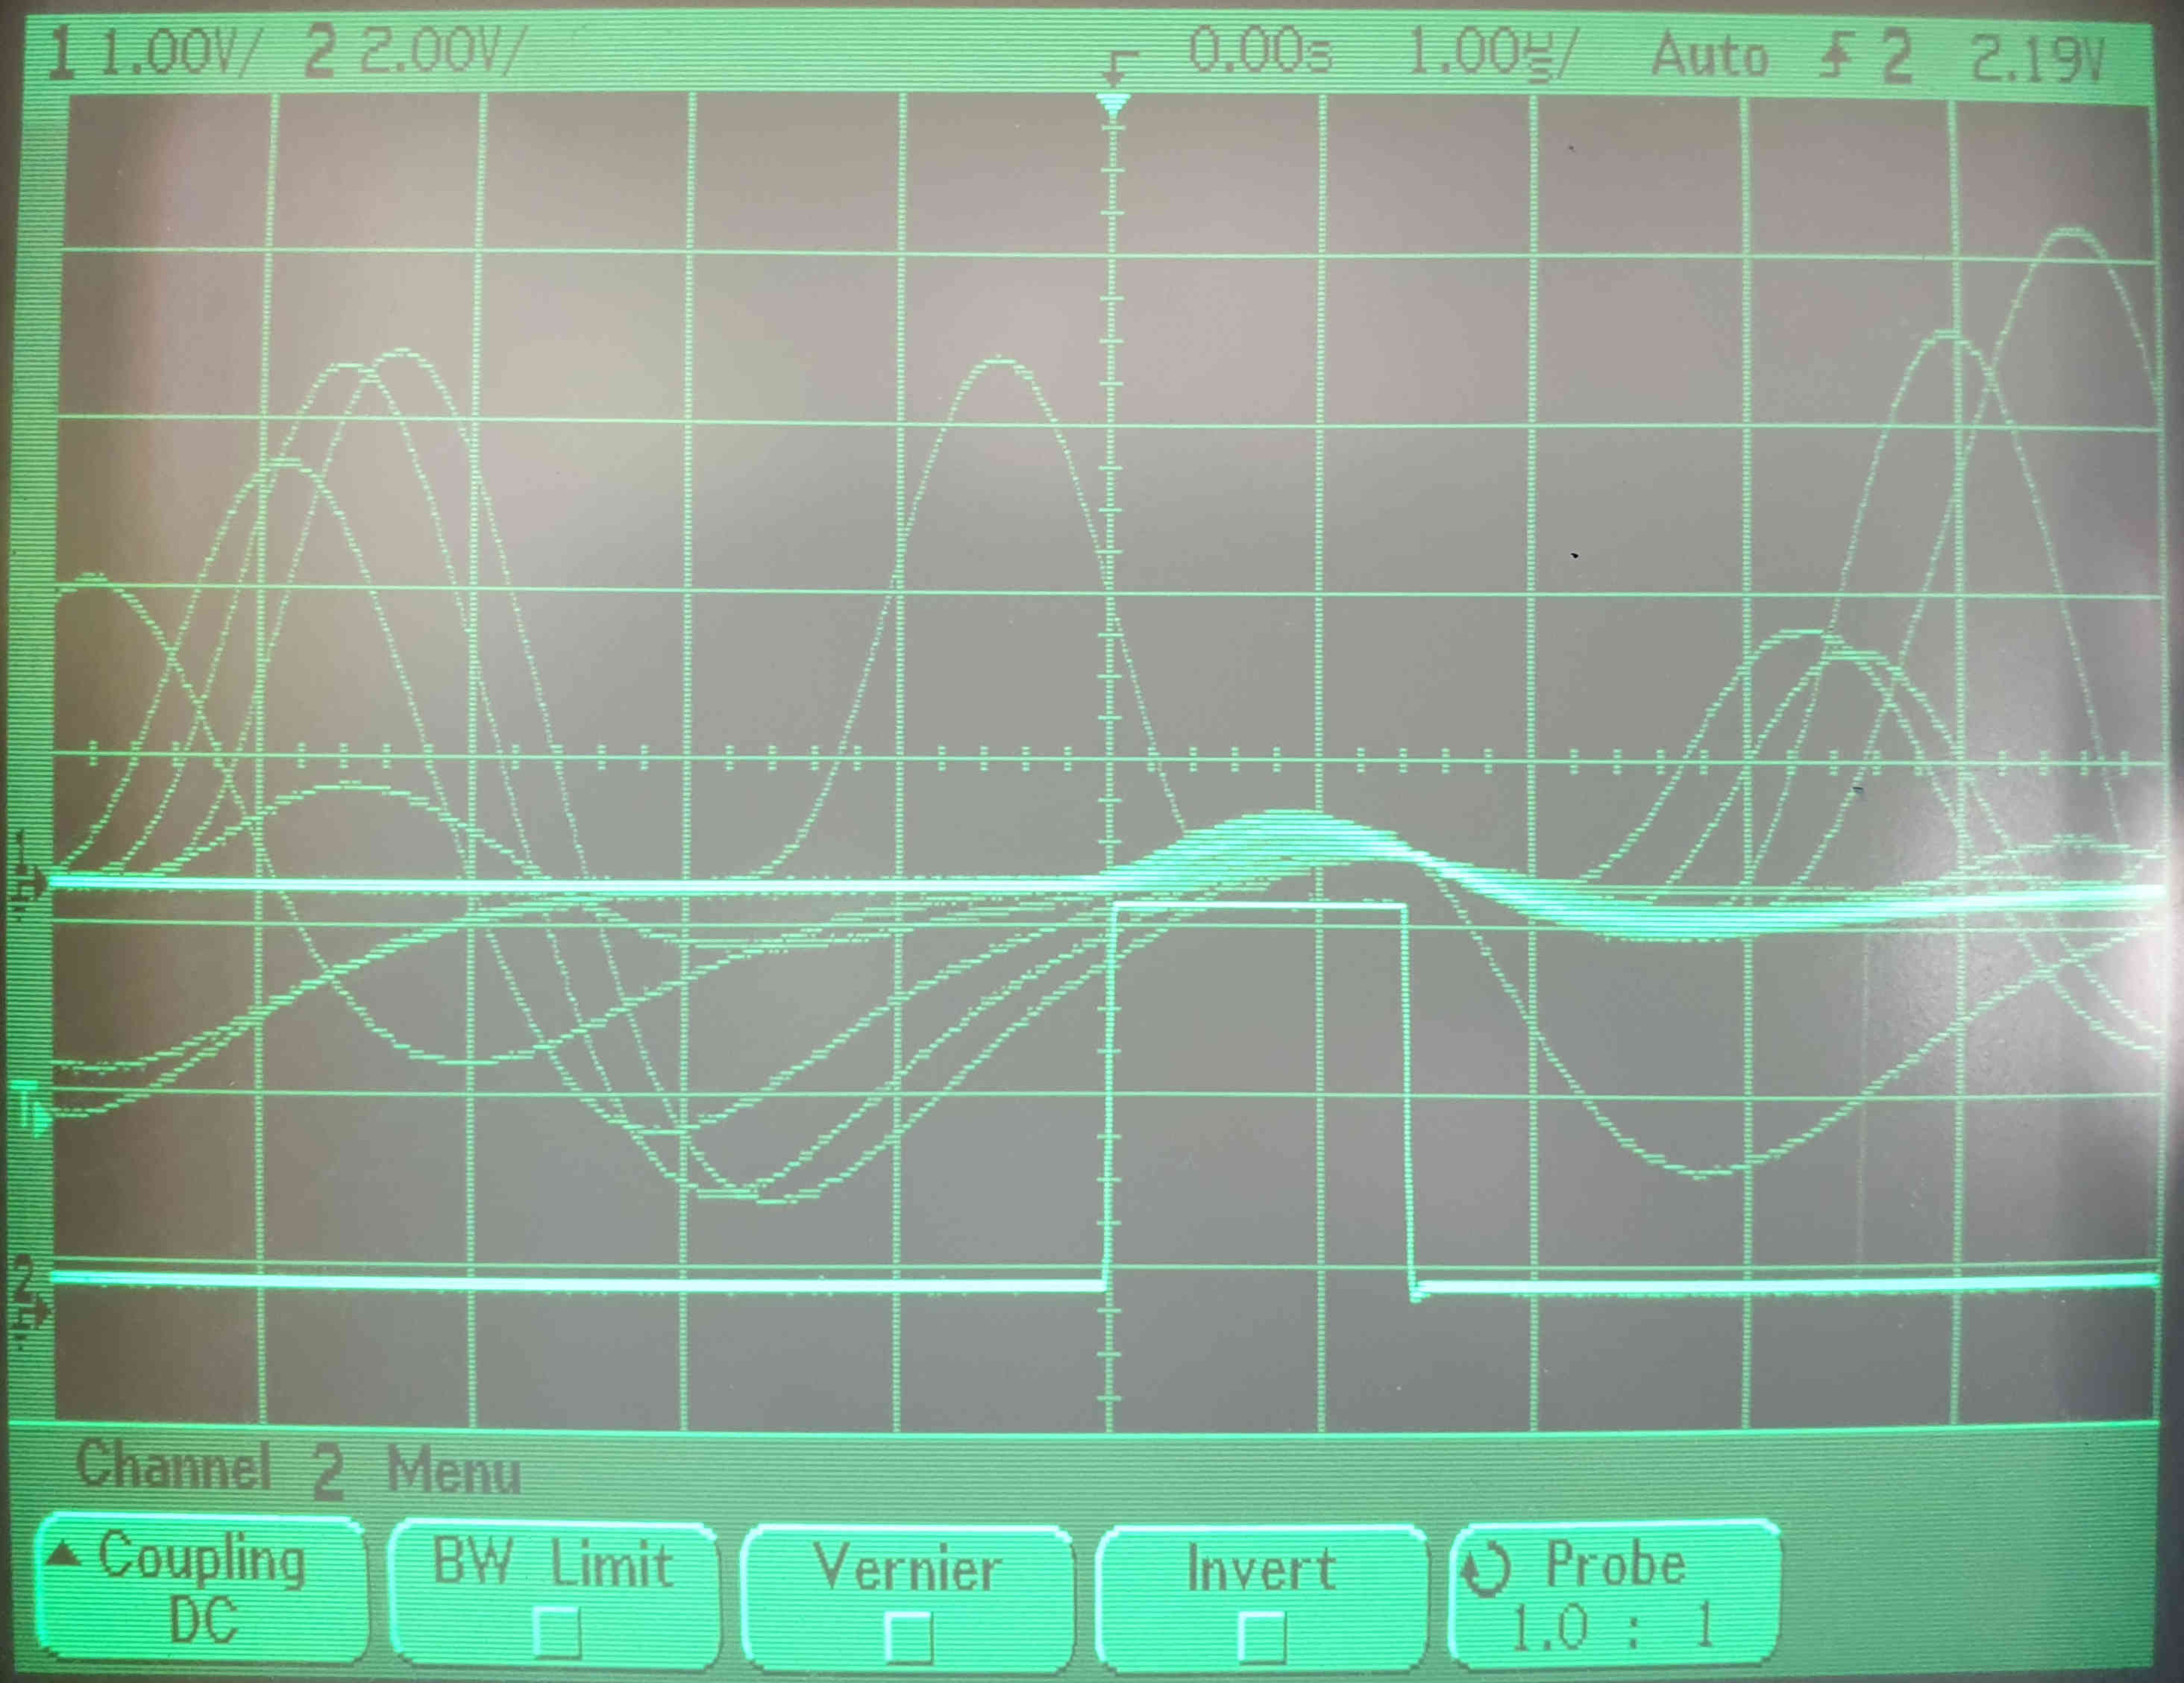
\includegraphics[width=\textwidth]{Bilder/1210_125430.jpg}
        \caption{Einstellung des Energiefensters auf die \SI{14,4}{\kilo\electronvolt} Linie}
    \end{subfigure}
    \caption{Einstellung des Energiefensters mithilfe des Oszilloskops. Die einzelnen Kurven in a.) zeigen die registrierten Signale für unterschiedliche Energien des $^{57}$Co-Spektrums.}
    \label{fig:Oszilloskop}
\end{figure}\\
Das Triggerlevel wird auf das \textit{SCA} Signal gelegt. Nun wird das lower level (E) am \textit{SCA} so eingestellt, dass es knapp über \SI{0}{\volt} liegt, um Rauschen zu vermeiden. Das Window $\Delta E$ wird anschließend so eingestellt, dass nur noch die unter der sich zwischen den Signalbergen auftuenden Lücke sichtbaren Linien dargestellt werden. Praktisch ist dies gut umzusetzen, indem das Signal so verschoben wird, dass die \SI{14,4}{\kilo\electronvolt} darstellende Linie (sich unterhalb der Lücke befindliche Linie) auf einem Orientierungsstrich des Oszilloskops liegt. Dann kann das Energiefenster $\Delta E$ so eingestellt werden, dass die Linien bis zu der vorher eingestellten Grenze abgeschnitten werden.

\paragraph{Einstellung mit Vielkanalanalysator}
Durch Triggerung des ADC über seinen Gate-Eingang kann die Wirkung der Fenstereinstellung am \textit{SCA} direkt am Vielkanalanalysator beobachtet und dadurch die Resonanzabsoprtionslinie genauer eingestellt werden. \\
Dazu wird der Output des \textit{Amplifiers} in den Eingang des \textit{SCA} und in den \textit{Delay Amplifier} eingegeben. Der Ausgang letzterem wird am Oszilloskop sichtbar gemacht. Der Output des \textit{SCA} wird in den \textit{Delay-Gate-Generator} eingegeben.
Auch hier wird der Output am Oszilloskop dargestellt. Jetzt werden die Einstellungen am \textit{Delay-Gate-Generator} und am Delay Amplifier so verändert, dass das Rechtecksignal genau die Breite der Erhebung des Energiesignals hat und die Flanken am Anfang bzw. am Ende der Erhebung liegen. Dazu wird am $t_d$ und $t_w$ Knopf des DGG gedreht und die Schalter des \textit{Delay Amplifiers} ein- bzw ausgeschalten. Nach der Optimierung der Einstellungen wird das Ausgangssignal des DGG an den Gate-Anschluss des ADC und das Ausgangssignal des \textit{Delay Amplifiers} an die PHA Buchse angelegt. Nun wird auf dem Vielkanalanalysator genau der Ausschnitt des Energiespektrums angezeigt, der die \SI{14,4}{\kilo\electronvolt} zeigt. Um einen kürzeren Ausschnitt zu sehen, wird $\Delta E$ kleiner eingestellt, um einen Ausschnitt höherer Energien zu sehen, wird das \textit{Lower Level} nach oben korrigiert. \\

\subsection{Messung und Auswertung von Mößbauerspektren}
Hierfür wird der Output des \textit{Amplifiers} in den \textit{SCA} eingegeben. Der Output des \textit{SCA} wird nach Einstellung des Fensters auf die \SI{14,4}{\kilo\eV} Linie - die vom \textit{SCA} erzeugten Pulse entsprechen nun dieser ausgewählten Energie - an den \textit{MCA} (\textit{Multi channel Analyzer}) Eingang des \textit{ADC} angeschlossen.
Die Messung erfolgt nach dem in Abbildung \ref{fig:BlockMoessbauerspektren} dargestellten Prinzip:
\begin{figure}[htp]\label{fig:BlockMossbauerspektren}
    \centering
    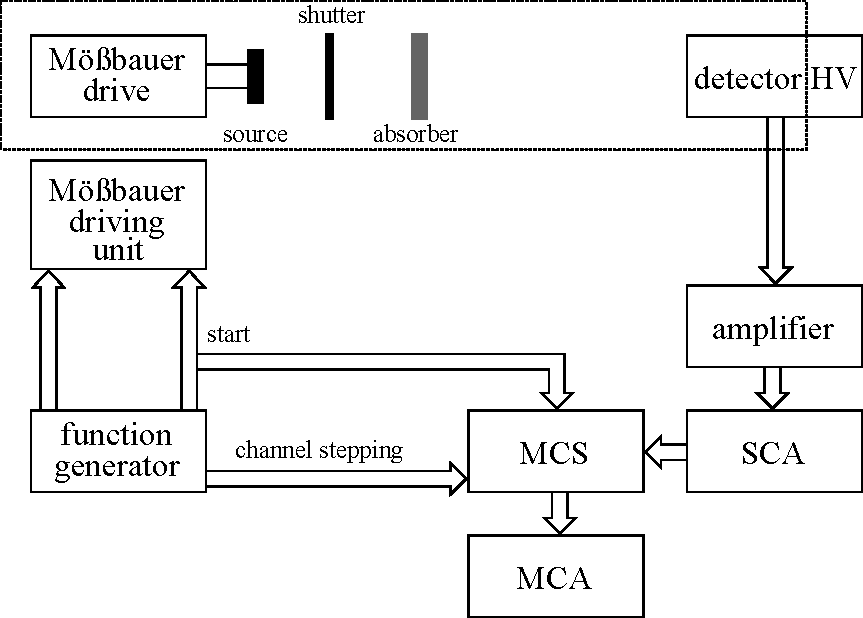
\includegraphics[width=0.7\textwidth]{Schaltungen/Blockschaltbild.pdf}
    \caption{Blockschaltbild zur Messung von Mößbauerspektren nach~\cite{Reisloehner}}
    \label{fig:BlockMoessbauerspektren}
\end{figure}

Im Versuch wird eine Transmissionsgeometrie verwendet. \textsuperscript{57}Co wird als radioaktive Quelle genutzt und mit dem Mössbauer Drive, einem lautsprecherähnlichen Antrieb, bewegt. Der Impulsgenerator gibt die Geschwindigkeit der Quelle vor, die im Versuch einem kosinusförmigen Verlauf folgt und über die \textit{Mössbauer Driving Unit} an den \textit{Mößbauer Drive} übertragen wird. Durch die oben beschriebenen Fenstereinstellungen ist gewährleistet, dass die vom \textit{SCA} erzeugten Pulse den Ereignissen der \SI{14,4}{\electronvolt}-Energie entsprechen. Diese werden von der Zähleinheit im \textit{MCS}-Modus (\textit{Multichannel Scaling}) registriert und im \textit{MCA} aufsummiert. Der Impulsgenerator gibt dabei Triggerpulse zur Weiterschaltung des Kanals, diese erfolgt in äquidistanten Zeitschritten, sowie zur Zurücksetzung der Kanalnummer bei $ v = v_\text{max} $ an den \texit{MSC}.  So ist es möglich zu messen, wie viele Ereignisse bei einer bestimmten Geschwindigkeit auftreten. Mit dem Messprogramm \glqq WISSOFT2003\grqq{} kann der Histogrammspeicher \textit{MCA} ausgelesen werden.
Das Mößbauerspektrum von natürlichem Eisen (Folienstärke \SI{25}{\micro\meter}), von Edelstahl und von Eisensulfat werden aufgenommen, indem der genannte Stoff jeweils als Absorber eingelegt wird.
% *********************************************
% ***** KAPITEL 4 *****************************
% *********************************************
\newpage
\section{Ergebnisse und Diskussion}
\subsection{Abschätzung einer oberen Strahlendosis}
Vor Beginn des Experiments wurde eine Abschätzung durchgeführt, wie groß die aufgenommene Äquivalentdosis $H$ im Verlauf des Versuchs maximal werden kann. Dabei wurde ein Abstand von \SI{1}{\metre} ohne Abschirmung gewählt. Es gilt folgende Formel:
\begin{align}
  H = \Gamma_H \frac{A t}{r^2}.
\end{align}
Die Aktivität $A$ der $^{60}$Co Quelle beträgt etwa \SI{200}{\kilo\becquerel}. Bei $\Gamma_H$ handelt es sich um eine Proportionalitätskonstante, es gilt $\Gamma_H(^{60}\text{Co})= \SI{351}{\micro\sievert\metre\squared\per\hour\per\giga\becquerel}$. Damit ergibt sich für eine Praktikumszeit von 12 Stunden eine Strahlendosis von
\begin{align}
  H = \SI[per-mode=fraction]{351}{\micro\sievert\metre\squared\per\hour\per\giga\becquerel} \cdot\frac{\SI{2e5}{\becquerel}\cdot\SI{12}{\hour}}{\SI{1}{\metre\squared}}= \SI{0,84}{\micro\sievert} \ll \SI{4}{\milli\sievert}.
\end{align}
Die Strahlendosis ist geringer als die täglich zulässige Strahlenbelastung und befindet sich im Größenbereich der statistischen Schwankungen der Radioaktivität. Die durch das Experiment aufgenommene Strahlendosis kann somit als unbedenklich eingestuft werden.

\subsection{Messung des Energiespektrums der $^{57}$Co-Quelle}
\subsubsection{Aufnahme verschiedener Energiespektren}
Zunächst wurden mithilfe des Programms \textit{WISSOFT2003} Energiespektren verschiedener Strahler aufgenommen. Dafür wurde eine Pulshöhenanalyse (PHA) durchgeführt. Die Gammastrahlung wird detektiert, digitalisiert und in einem, der Impulshöhe entsprechenden, Kanal abgelegt. Die Messung verlief jeweils über mehrere Minuten. Die Spektren der drei verwendeten Strahler sind in Abbildung~\ref{fig:Energiespektren} dargestellt.
\begin{figure}[htp]
    \vspace{-0.5cm}
    \centering
    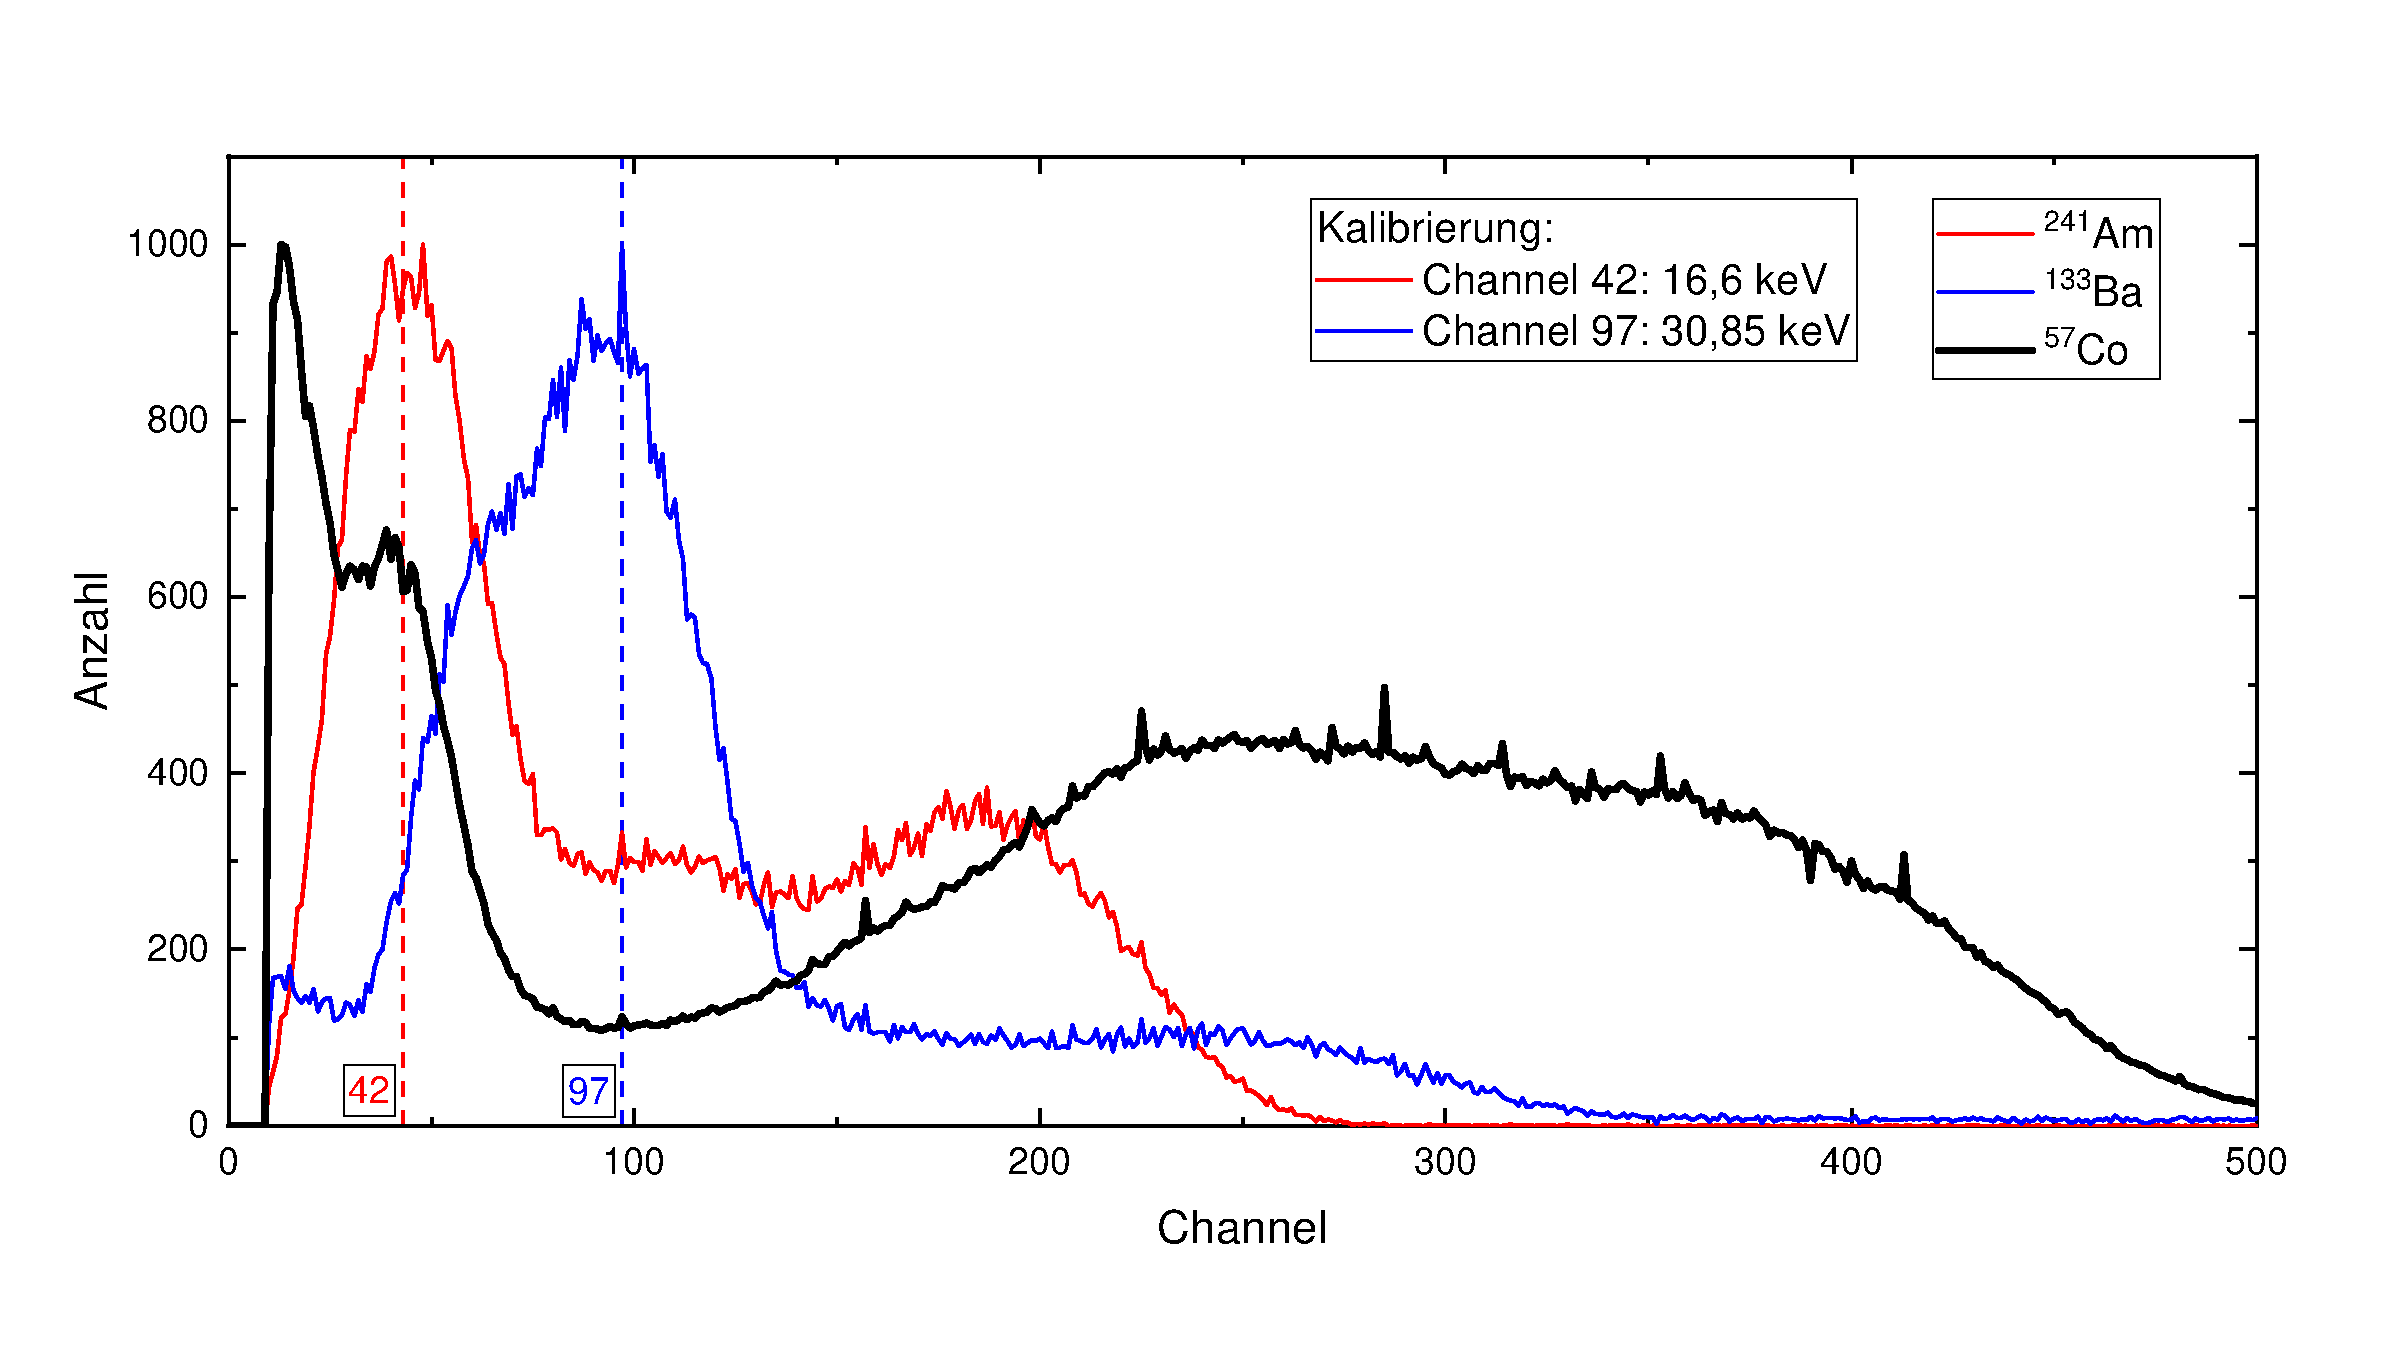
\includegraphics[width=0.95\textwidth]{Bilder/Energiespektren_Am_Ba_Co.pdf}
    \caption{Energiespektren der drei überprüften radioaktiven Quellen. Die Messwerte wurden auf eine Zahl von 1000 \glqq normiert\grqq.}
    \label{fig:Energiespektren}
\end{figure}
\subsubsection{Identifizierung der \SI{14,4}{\kilo\electronvolt} Linie}
Mithilfe der am Versuchsplatz vorhandenen Datenblätter wird mithilfe der Energiespektren von $^{241}$Am (Americium) und $^{133}$Co (Kobalt) eine Energiekalibrierung durchgeführt. Dafür wird der Kanal der bekannten Spektrallinie dieser Isotope identifiziert und auf die zugehörige Energie kalibriert. Für Barium befand sich die \SI{30,85}{\kilo\electronvolt} Linie bei Channel 97 und bei Americium die \SI{16,6}{\kilo\electronvolt} Linie bei Channel 42. Nun erfolgt eine erneute Aufnahme des Kobaltspektrums, woraus ein Ausschnitt in Abbildung~\ref{fig:Spektrum_Co} dargestellt ist.
\begin{figure}[htp]
    \vspace{-0.5cm}
    \centering
    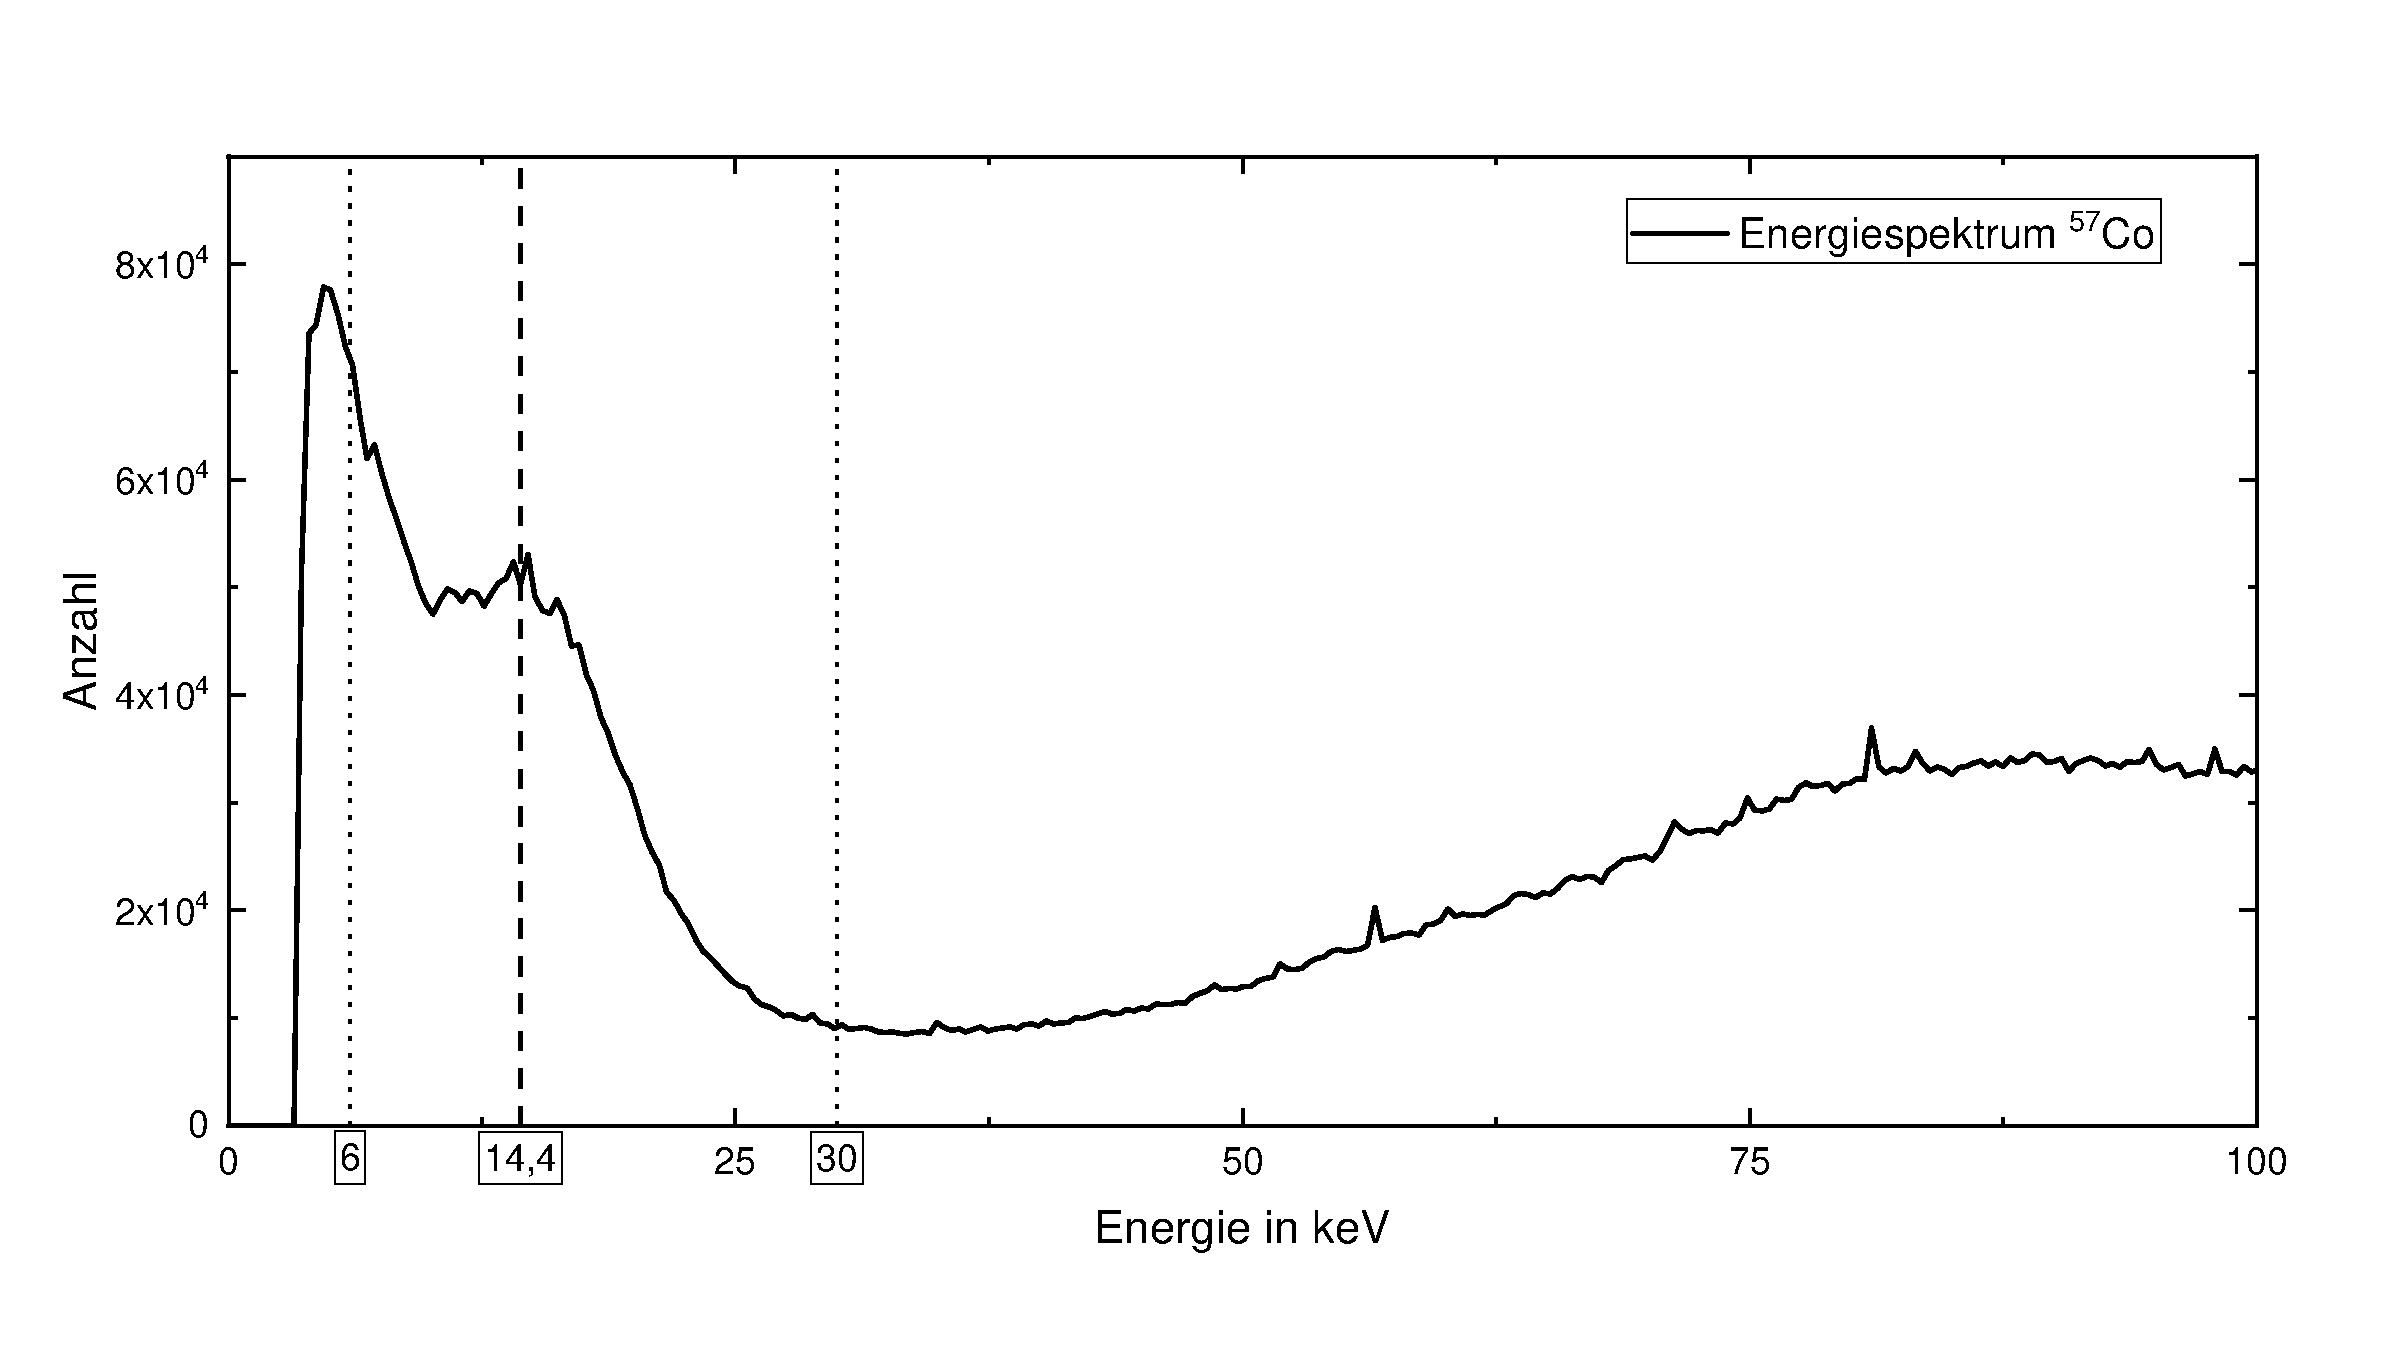
\includegraphics[width=0.95\textwidth]{Bilder/Energiespektrum_Co_kalibriert.pdf}
    \caption{Energiespektrum der $^{57}$Co Quelle mit kalibrierter Skala zur Identifizierung der \SI{14,4}{\kilo\electronvolt} Linie.}
    \label{fig:Spektrum_Co}
\end{figure}\\
Die bereits in Abschnitt~\ref{sec:Energiefenster} beschriebene Einstellung des Energiefensters mithilfe des Oszilloskops beeinflusst das resultierende Energiespektrum. Damit nur dann ein Signal übertragen wird, wenn ein \SI{14,4}{\kilo\electronvolt} Übergang stattfand, wird das Energiefenster so gewählt, dass nur die gesuchte Linie auftaucht. Für die folgenden Messungen wurde das in Abbildung~\ref{fig:Spektrum_Co} dargestellte Fenster zwischen ca. $6-\SI{30}{\kilo\electronvolt}$ gewählt.

\subsection{Auswertung der Mößbauerspektren}
\subsubsection{Spektrum von Eisen}
Zur Aufnahme des Mößbauerspektrums wurde als Absorber Eisen mit einer Folienstärke von $d = \SI{25}{\micro\metre}$ gewählt. Mithilfe des \textit{Mößbauer Drive} wird die radioaktive Quelle bewegt. Zunächst erfolgt eine Testaufnahme von $\SI{20}{\min}$, um eine passende maximale Probengeschwindigkeit zu ermittelt. Nun wird an der Steuereinheit eine maximale Probengeschwindigkeit von $v_\text{max} = \SI{5,99}{\milli\metre\per\second}$ eingestellt und die Messung 8 Stunden lang durchgeführt. Es ergibt sich nun ein Transmissionsspektrum über 1024 Kanäle. Dabei folgt die zugehörige Geschwindigkeit der Kanäle einem Kosinus. Mithilfe der Formel
\begin{align}
  v(n) = -\cos\left(\frac{n\cdot2\pi}{N}\right), \quad N = 1024
\end{align}
wurde die zugehörige Geschwindigkeit zum Kanal $n$ berechnet. Die Werte gleicher Geschwindigkeit wurden anschließend aufaddiert und es ergibt sich das in Abbildung~\ref{fig:Spektrum_Eisen} dargestellte Spektrum.
\begin{figure}[htp]
    \centering
    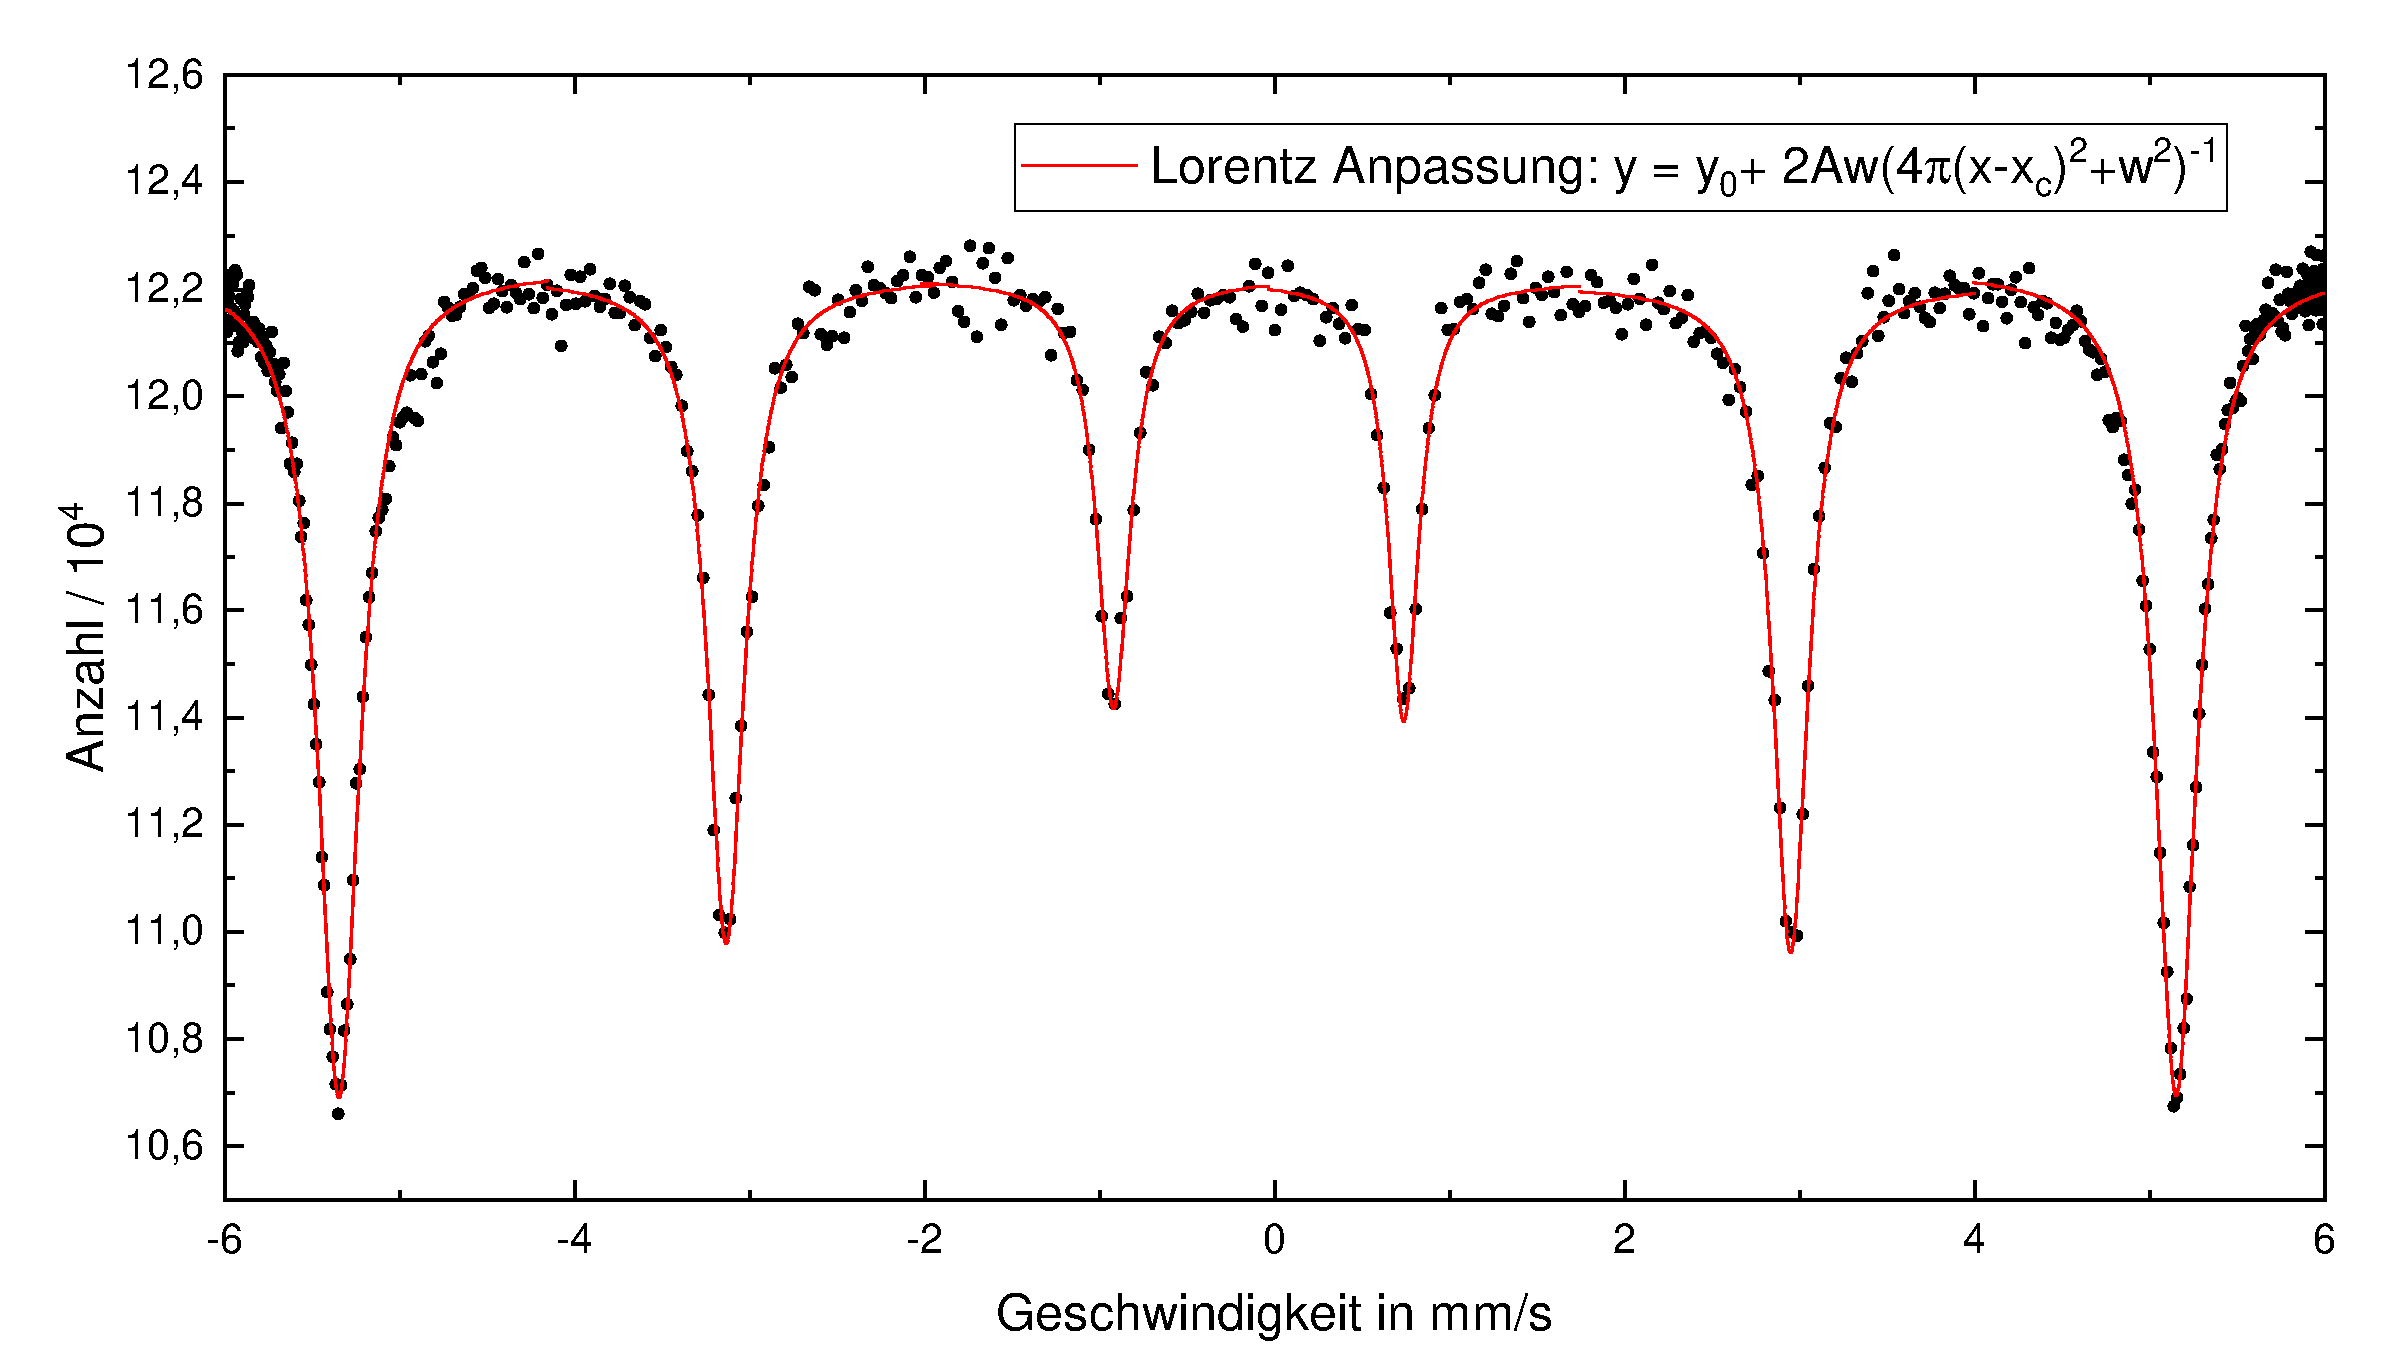
\includegraphics[width=0.95\textwidth]{Bilder/Moessbauer_Fe25_Lorentz.pdf}
    \caption{Mößbauerspektrum von Eisen.}
    \label{fig:Spektrum_Eisen}
\end{figure}\\
Das beobachtete Transmissionsspektrum besteht aus sechs annähernd symmetrisch zur Ruhelage liegenden, äquidistanten Absorptionslinien. Diese Linien werden durch die magnetische Wechselwirkung des Kerns mit einem äußeren $\bm{B}$-Feld verursacht, was zu einer Hyperfeinstrukturaufspaltung führt. Das Intensitätsverhältnis der Linien beträgt etwa $1:2:3$, was auf eine unmagnetisierte Probe schließen lässt.
Die einzelnen Absorptionslinien wurden in \textit{Origin} mithilfe eines Lorentzfits der Form
\begin{align}
  y= y_0 + \frac{2A}{\pi}\frac{w}{4(x-x_c)^2+w^2}\label{eqn:Lorentzfits}
\end{align}
an die Messdaten angepasst. Aus der Fitfunktion wurde die durch den Parameter $x_c$ die Position der Absorptionslinie bestimmt. Die in Abbildung~\ref{fig:Spektrum_Eisen} abgebildeten Absorptionslinien entsprechen von links nach rechts in aufsteigender Reihenfolge der Energieaufspaltung im Eisen. Dies lässt sich dadurch begründen, dass sich bei einer negativen Geschwindigkeit die Probe vom Absorber wegbewegt und dadurch nach Gleichung~\eqref{eqn:Dopplereffekt} eine \glqq Rotverschiebung\grqq{} aufgrund des Dopplereffekts auftritt und somit die Energie der Gammastrahlung sinkt. Analog dazu tritt bei positiver Geschwindigkeit eine \glqq Blauverschiebung\grqq{} auf. Alle möglichen Übergänge sind in Abbildung~\ref{fig:Termschema_Eisen} dargestellt. Dabei wurden die Auswahlregeln $\Delta l = \Delta J = \pm 1$ und $\Delta M = 0; \pm 1$ beachtet.
\begin{figure}[htp]
    \centering
    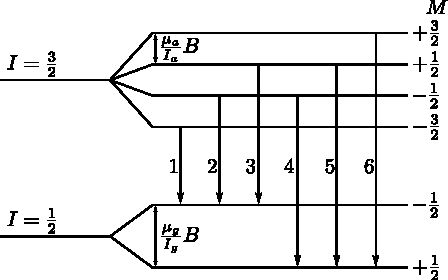
\includegraphics{Bilder/Termschema_Eisen.pdf}
    \caption{Das Termschema von Eisenkernen in einem $\bm{B}$-Feld. Alle möglichen Übergänge sind nach den Auswahlregeln $\Delta l = \pm 1 , \Delta M = 0; \pm 1$ nach aufsteigender Energie sortiert (eigene Abbildung nach~\cite{Schatz}).}
    \label{fig:Termschema_Eisen}
\end{figure}\\
Um nun daraus die Energieaufspaltung im Grundzustand $\Delta E_g$ bzw. im angeregten Zustand $\Delta E_a$ zu bestimmen, müssen die Energien bestimmter Übergänge voneinander subtrahiert werden. Für die Energieaufspaltung des Grundzustandes werden zwei Übergänge vom gleichen angeregten Zustand in zwei unterschiedliche Grundzustände benötigt. Dies ist bei Übergang 2 und 4, sowie 3 und 5 der Fall. Zur Berechnung der Aufspaltung der angeregten Zustände werden zwei Übergänge aus unterschiedlichen angeregten Zuständen in den gleichen Grundzuststand benötigt, wie beispielsweise bei Übergang 1 und 2.\\
Zunächst wird aus den gewonnenen Geschwindigkeiten mithilfe von \eqref{eqn:Dopplereffekt} die Energiedifferenz zu einer Bezugsgröße bei $v = \SI{0}{\milli\metre\per\second}$ bestimmt
\begin{align}
  \Delta E &= \hbar \omega - \hbar \omega_0 = \hbar k v, \quad k = \frac{\omega}{c} = \frac{E}{\hbar c}\\
  \Rightarrow \Delta E &= v\frac{E}{c}.\label{eqn:Energieaufspaltung}
\end{align}
Für die Energie wird $E = \SI{14,4}{\kilo\electronvolt}$ verwendet. Die Ergebnisse dieser Rechnungen sind ausführlich in Tabelle~\ref{tab:Energieaufspaltung_Eisen} zusammengefasst.
\begin{table}[ht]
	\centering
	\caption{Auswertung der Absorptionslinien von Eisen und Bestimmung Energieaufspaltung. Die Geschwindigkeit $v$ wurde aus dem Parameter $x_c$ der Lorentzanpassung gewonnen. $\Delta E_g$ bezeichnet die Energieaufspaltung des Grundzustandes und $\Delta E_a$ die Aufspaltung der angeregten Zustände.}
	\label{tab:Energieaufspaltung_Eisen}
  \begin{tabular}{c S[table-format=-1.4(5),separate-uncertainty] S[table-format=-3.2(3), separate-uncertainty] c S[table-format=3.2(3),separate-uncertainty] S[table-format=3.2(3),separate-uncertainty]}
  \toprule
  Nr. &{$v$ [\si{\milli\metre\per\second}]} & {$E-E_0$ [\SI{e-9}{\electronvolt}]} & Übergang & {$\Delta E_g$ [\SI{e-9}{\electronvolt}]} &{$\Delta E_a$ [\SI{e-9}{\electronvolt}]}\\
   \midrule
  1 & -5.3492 +- 0.0016 & -256.94 +- 0.07 & $E_2-E_1$ &               &  106.31 +- 0.18 \\
  2 & -3.1359 +- 0.0022 & -150.63 +- 0.10 & $E_3-E_2$ &               &  106.33 +- 0.27\\
  3 & -0.9223 +- 0.0036 & -44.30  +- 0.17 & $E_4-E_2$ & 185.96 +- 0.27           &        \\
  4 & 0.7357  +- 0.0034 & 35.34   +- 0.16 & $E_5-E_3$ & 185.83 +- 0.28           &        \\
  5 & 2.9466  +- 0.0022 & 141.53  +- 0.11 & $E_5-E_4$ &               &  106.20 +- 0.27\\
  6 & 5.1499  +- 0.0014 & 247.37  +- 0.07 & $E_6-E_5$ &               &  105.83 +- 0.27\\ \bottomrule
  \end{tabular}
\end{table}\\
Durch Mittelung der berechneten Werte und Berechnung der Standardabweichung ergeben sich folgende Werte für die Energieaufspaltung:
\begin{align}
  \Delta E_g &= \SI[separate-uncertainty]{185,90 \pm 0,22 e-9}{\electronvolt}\\
  \Delta E_a &= \SI[separate-uncertainty]{106,17 \pm 0,24 e-9}{\electronvolt}.
\end{align}
\paragraph{Magnetfeld und magnetisches Moment}$~$\\
Aus den gewonnenen Werten für die Aufspaltung des Grundzustandes lässt sich nun mithilfe von Gleichung~\eqref{eqn:Magnetfeld} das Magnetfeld $B$ am Ort der $^{57}Fe$-Kerne berechnen. Es folgt mit dem magnetischen Kernmoment
\begin{align}
  \mu_K = \frac{e}{2m_p}\hbar = \SI[per-mode=fraction]{5,050783e-27}{\joule\per\tesla}
  \end{align}
und $J_g = \frac{1}{2}$ im Grundzustand die Formel für das Magnetfeld
  \begin{align}
  \Rightarrow B = -\frac{\Delta E_g I_g}{\mu_g} = -\frac{\Delta E_g I_g}{0,0906\cdot\mu_K} = \SI[separate-uncertainty]{-32,54 \pm 0,04}{\tesla}.
  \end{align}
Das negative Vorzeichen bedeutet, dass das $\bm{B}$-Feld und die äußere Magnetisierung der Probe entgegengesetzt zueinander orientiert sind. Für das magnetische Moment des angeregten Zustands ergibt sich mit $I_a = \frac{3}{2}$ analog nun
  \begin{align}
  \mu_a &= \frac{\Delta E_a I_a}{B} = \SI[per-mode=fraction]{-0,7840 \pm 0,0027e-27}{\joule\per\tesla}\\
  &= \SI[separate-uncertainty]{-0,1552\pm 0,0005}{\micro_K}
\end{align}
Die in der Literatur~\cite{Schatz} (S.71) angegebenen Werte lauten
\begin{align}
  B &= \SI[separate-uncertainty]{-33,3 \pm 1,0}{\tesla}\\
  \mu_a &= \SI[separate-uncertainty]{0,153\pm 0,004}{\micro_K}.
\end{align}
Somit liegen die gemessenen Werte innerhalb der Fehlertoleranzbereichs der Literaturwerte.
\paragraph{Isomerieverschiebung und Linienbreite}$~$\\
Die Isomerieverschiebung ist eine Relativgröße, weshalb immer eine Bezugssubstanz angegeben werden muss. In diesem Fall nimmt die Quelle die Rolle der Bezugssubstanz ein. Die Isomerieverschiebung bewirkt eine Verschiebung der Symmetrielage des Mößbauerspektrums gegenüber des Nullpunktes. Zur Berechnung der Verschiebung wird das arithmetische Mittel zwischen zwei symmetrisch gegenüberliegenden Linien des Spektrums gebildet, was grafisch in Abbildung~\ref{fig:Eisen_Isomerieverschiebung} dargestellt ist.
\begin{figure}[htp]
    \centering
    \vspace{-0.3cm}
    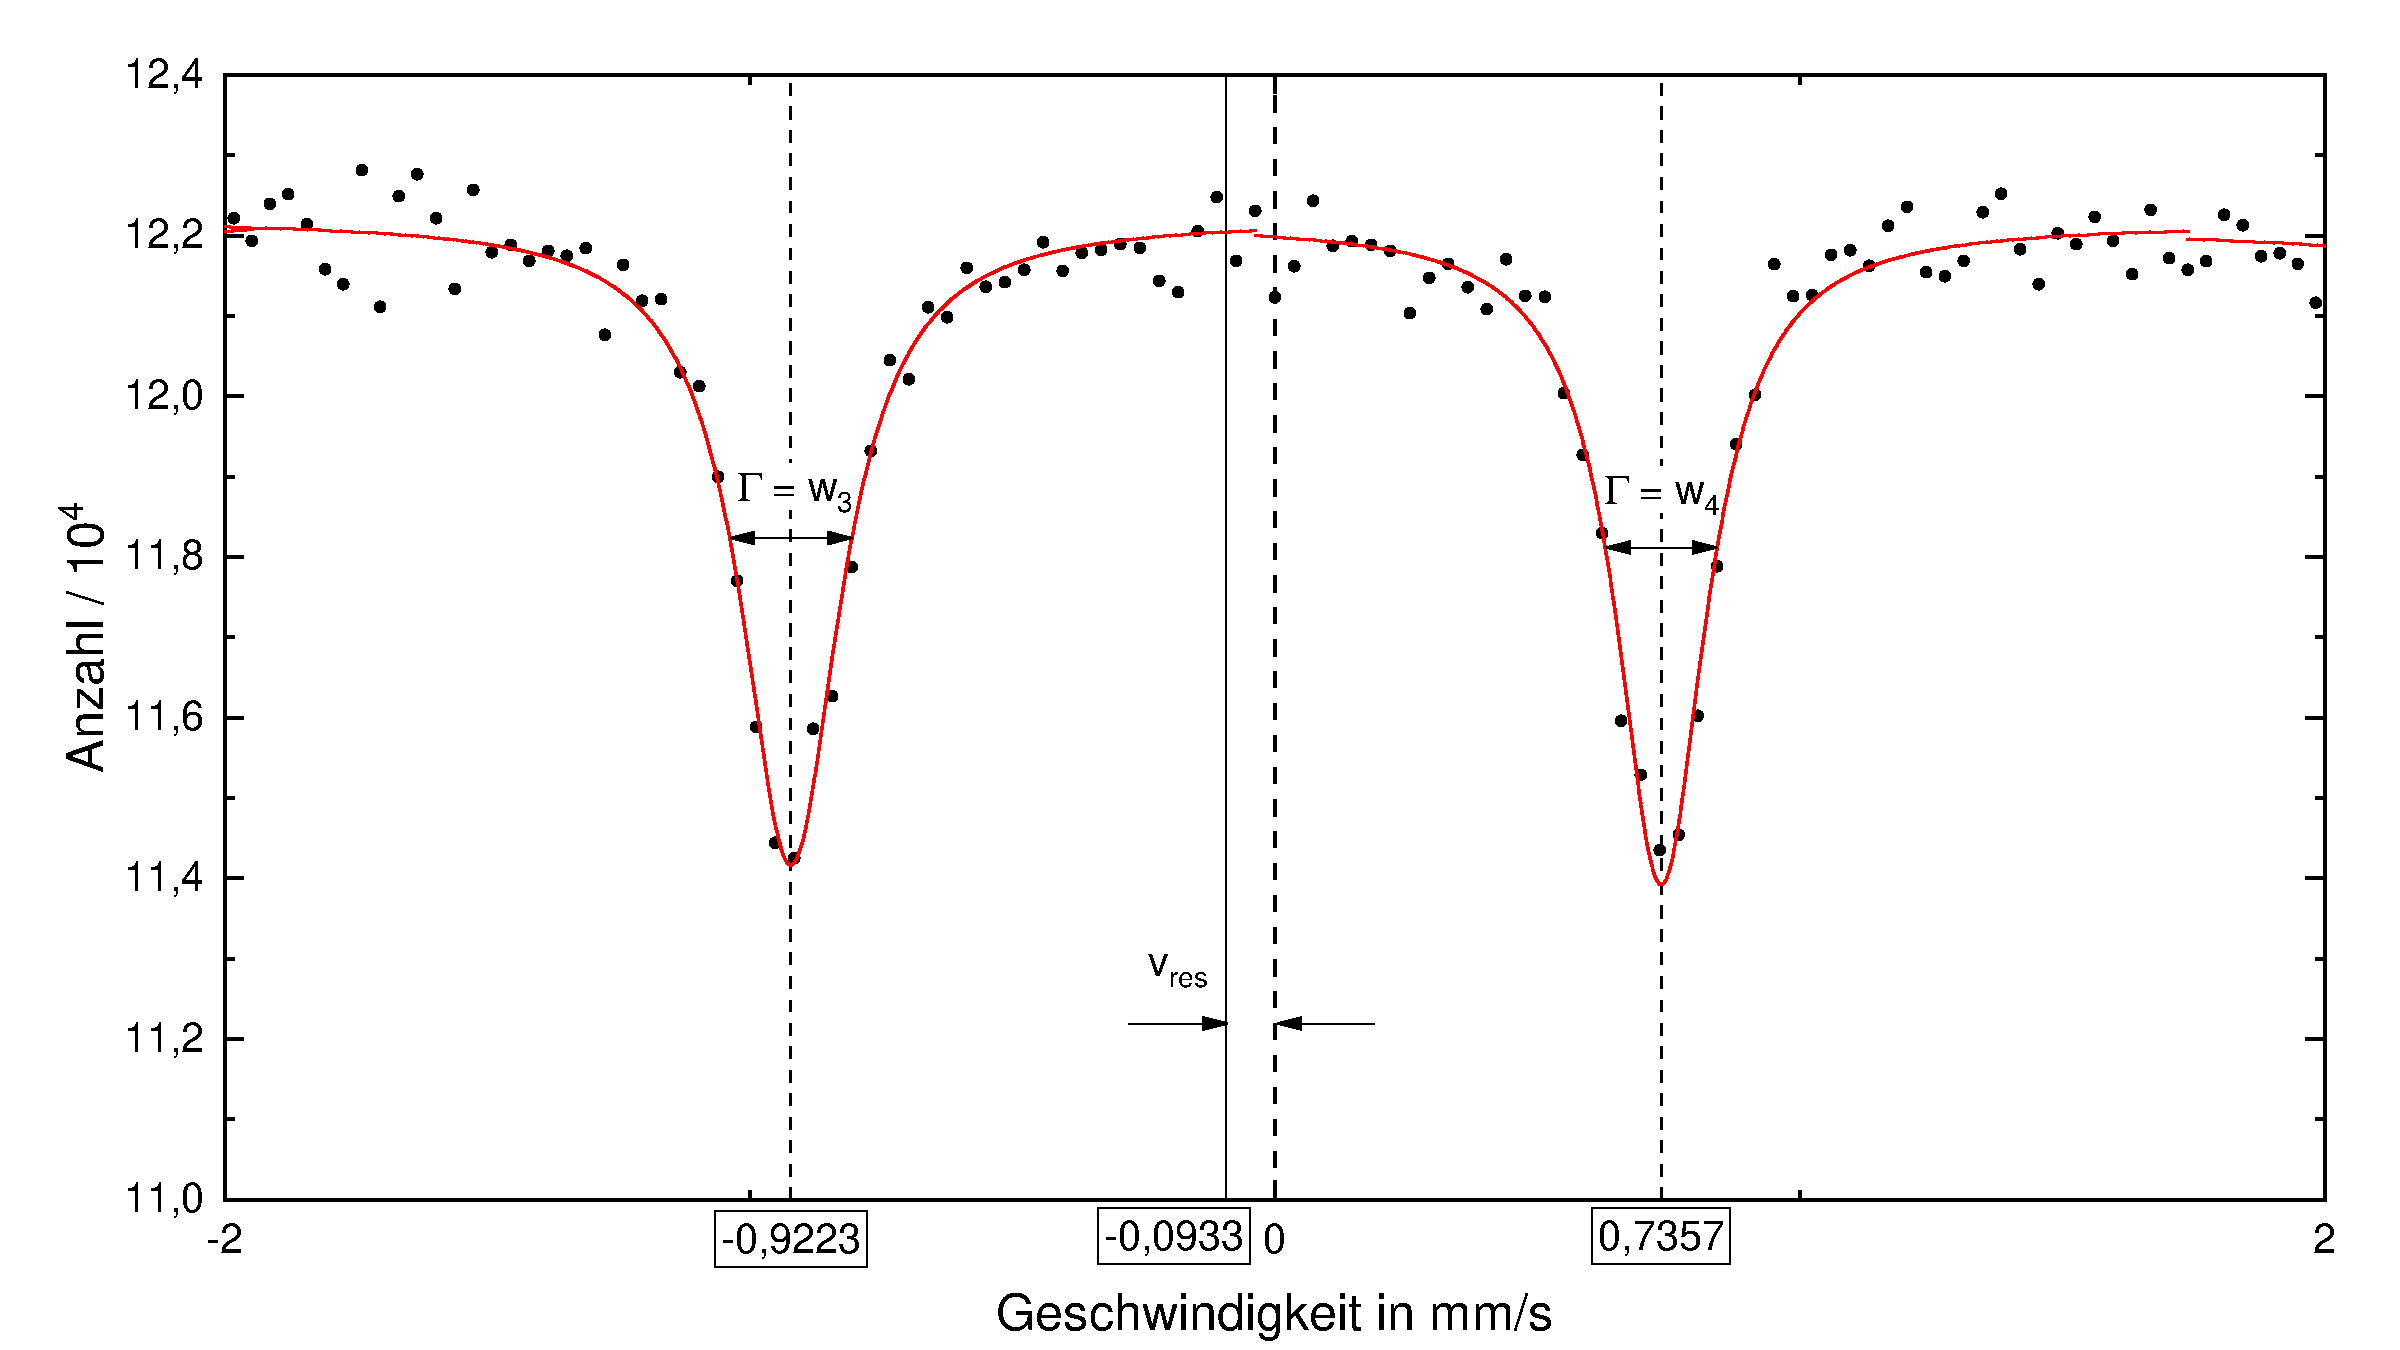
\includegraphics[width=0.95\textwidth]{Bilder/Eisen_Isomerieverschiebung.pdf}
    \caption{Grafische Veranschaulichung der Isomerieverschiebung des Mößbauerspektrums von Eisen und Ermittlung der Linienbreite der Absorptionslinien.}
    \label{fig:Eisen_Isomerieverschiebung}
\end{figure}\\
Zur Ermittlung der Linienbreite wird der Parameter $w$ der Lorentzanpassung \eqref{eqn:Lorentzfits} benötigt. Dieser gibt die Halbwertsbreite FWHM (\textit{Full Width at Half Maximum}) an und repräsentiert direkt die Linienbreite $\Gamma$. Die gemessene Isomerieverschiebung und Linienbreiten sind in Tabelle~\ref{tab:Isomerieverschiebung_Eisen} dargestellt.
\begin{table}[ht]
	\centering
	\caption{Bestimmung der Isomerieverschiebung und der Linienbreite der Absorptionslinien von Eisen.}
	\label{tab:Isomerieverschiebung_Eisen}
  \begin{tabular}{c S[table-format=-1.4(5),separate-uncertainty] S[table-format=-1.2(3),separate-uncertainty] c  S[table-format=1.3(4), separate-uncertainty] S[table-format=2.2(3),separate-uncertainty]}
  \toprule
  {Linien} & {$v_\text{res}$ [\si{\milli\metre\per\second}]} & {$v_\text{res}$ [\SI{e-9}{\electronvolt}]} & {Nr.} & {$v_\text{Linie}$ [\si{\milli\metre\per\second}]} & {$E_\text{Linie}$ [\SI{e-9}{\electronvolt}]}\\
   \midrule
  1 und 6 & -0.0997 \pm 0,0030& -4,79 \pm 0,14  &1  & 0,291 \pm 0,006     & 13,98 \pm 0,28 \\
          &                   &                 &2  & 0,258 \pm 0,008    &12,39 \pm 0,36 \\
  2 und 5 & -0,0947 \pm 0,0044 & -4,55\pm 0,21  &3   &0,230 \pm 0,012     & 11,02 \pm 0,59 \\
          &                   &                 &4  & 0,209 \pm 0,012    &10,04 \pm 0,57 \\
  3 und 4 & -0,0933 \pm 0,0070 & -4,48 \pm 0,33 &5  &0,250 \pm 0,008     & 12,01 \pm 0,37 \\
          &                   &                 &6  & 0,287 \pm 0,005    &13,77 \pm 0,24 \\
  \midrule
  \addlinespace
  \textbf{Mittelwert}  & -0,0959 \pm 0,0259 & -4,61	\pm 1,25
& & 0,254 \pm 0,073 & 12,20  \pm3,50 \\ \bottomrule
  \end{tabular}
\end{table}\\
Bei dem Vergleich der Linienbreiten fällt eine Zunahme der Breite für betragsmäßig größere Geschwindigkeiten auf.
%%%
%%% WARUM????
%%%
Die natürliche Linienbreite ist bestimmt durch die \textsc{Heisenberg}'sche Unschärferelation, wonach das Produkt aus Zeit- und Energieunschärfe gleich dem reduzierten \textsc{Planck}'schen Wirkungsquantum sind. Die Linienbreite $\Gamma$ stellt die Energieunschärfe dar. Wird die Zeitunschärfe als die mittlere Lebensdauer des Kernzustandes identifiziert, folgt
\begin{align}
  \Gamma \Delta t \ge \hbar \Rightarrow \Gamma = \frac{\hbar}{\tau_N}.
\end{align}
Nach dem Zerfallsschema~\ref{fig:Zerfallsschema} besitzt der Kernzustand eine Halbwertszeit von \SI{98}{\nano\second}, wodurch sich die Linienbreite zu
\begin{align}
  \Gamma = \hbar \frac{\ln 2}{t_{1/2}}= \SI{4.66e-9}{\electronvolt}, \quad t_{1/2} = \tau_n \ln 2
\end{align}
ergibt. Diese Linienbreite erfasst jedoch nur die Quelle, der Absorber besitzt (im Spezialfall von Eisen) die gleiche Linienbreite, wodurch sich das Ergebnis verdoppelt zu $\Gamma = \SI{9.32e-9}{\electronvolt}$. Der Grund, warum die gemessene Linienbreite größer ist, liegt an der endlichen Dicke der Probe. Mit steigender Probendicke nimmt ebenfalls die Linienbreite zu.

\subsubsection{Spektrum von Edelstahl}
Die Aufnahme des Mößbauerspektrums von Edelstahl erfolgte auf analoge Art und Weise mit einer Messdauer von 20 Stunden, allerdings wurde eine maximale Geschwindigkeit des Mößbauerantriebs von $v_\text{max} = \SI{2,41}{\milli\metre\per\second}$ eingestellt, da im Spektrum nur ein Absorptionslinie auftaucht. Es lässt sich also keine magnetische Aufspaltung erkennen. Das Spektrum ist in Abbildung~\ref{fig:Edelstahl_Spektrum} dargestellt.
\begin{figure}[htp]
    \centering
    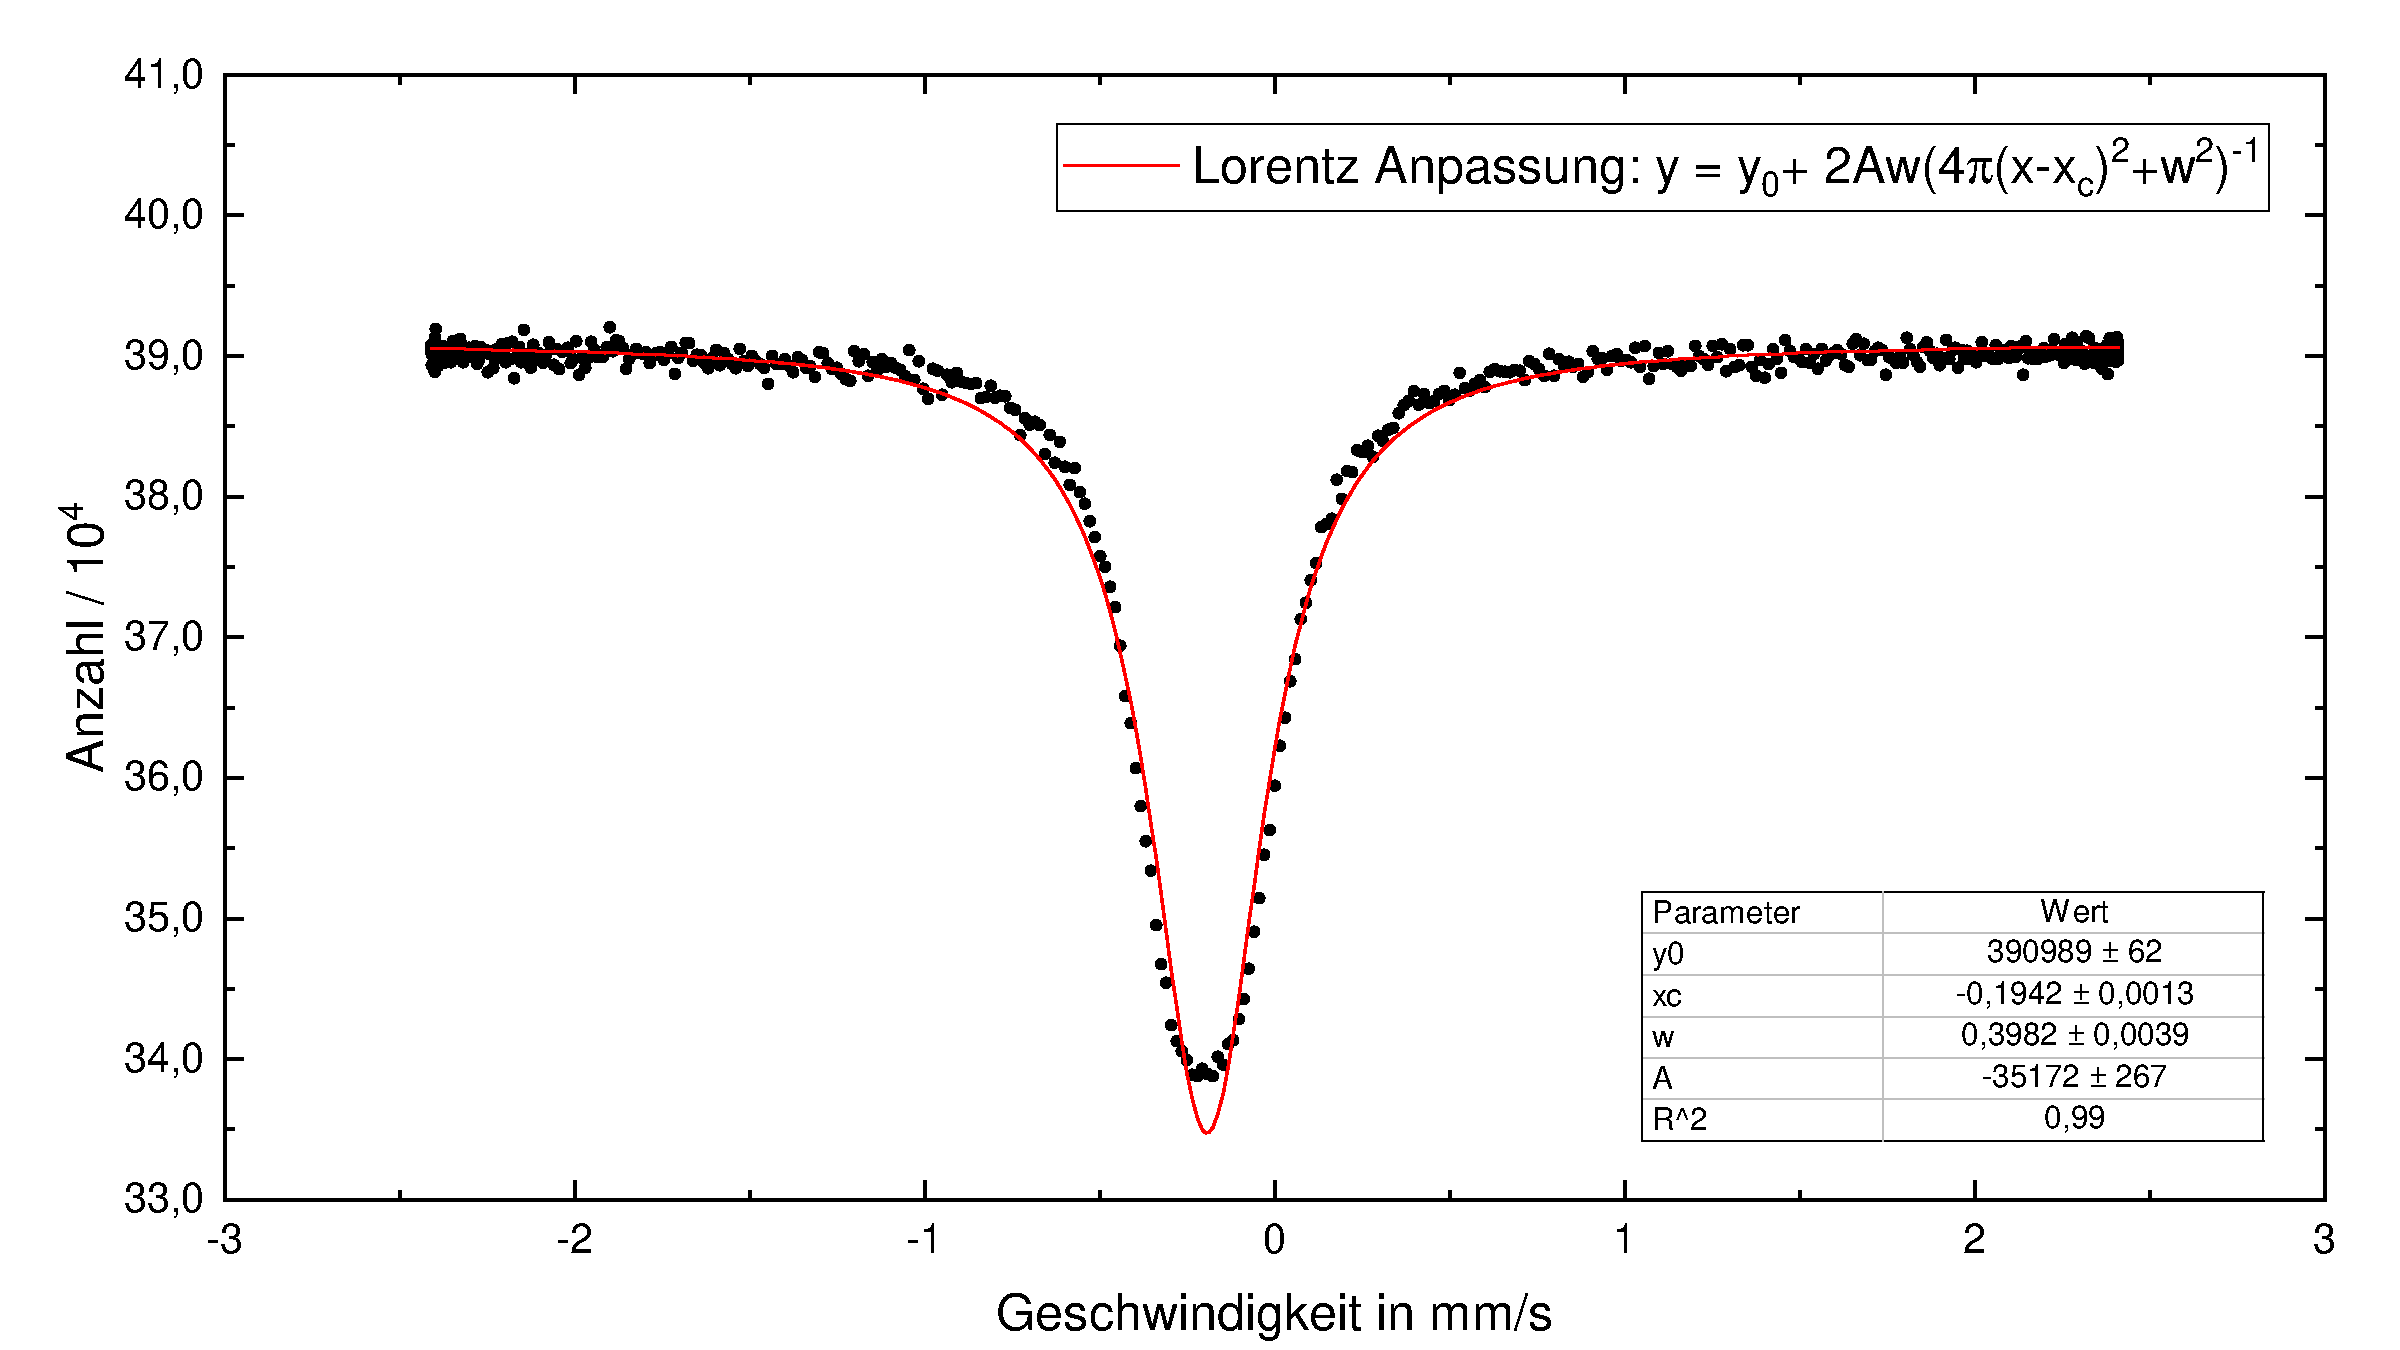
\includegraphics[width=0.95\textwidth]{Bilder/Moessbauer_Edelstahl_Lorentz.pdf}
    \caption{Mößbauerspektrum von Edelstahl. Es wurde wieder eine Lorentzanpassung der Form~\eqref{eqn:Lorentzfits} vorgenommen.}
    \label{fig:Edelstahl_Spektrum}
\end{figure}\\
Es lässt sich wieder die Isomerieverschiebung als die Verschiebung der Absorptionslinie zum Nullpunkt ablesen. Es ergibt sich
\begin{align}
  v_\text{res} &= \SI[per-mode=fraction, separate-uncertainty]{-0,1942\pm 0,0013}{\milli\metre\per\second}\\
  E_\text{res} &= \SI[separate-uncertainty]{-9,33
\pm 0,06}{\electronvolt}.
\end{align}
Bei Edelstahl handelt es sich um eine Legierung, weshalb die Eisen-Atome in unterschiedlicher chemischer Bindung vorliegen. Deshalb treten verschiedene Isomerieverschiebungen auf. Jedoch liegen diese so dicht beieinander, dass sie aufgrund der natürlichen Linienbreiten nicht als einzelne Absorptionslinien identifizierbar sind. Die bestimmte Isomerieverschiebung stellt deshalb einen Effektivwert dar. Trotzdem führt dies zu einer Verbreiterung der Linienbreite. Aus den Fitparametern lässt sich diese zu
\begin{align}
  v_\text{Linie} = \SI[per-mode=fraction, separate-uncertainty]{0,3982 \pm 0,0039}{\milli\metre\per\second}
\end{align}
bestimmen und ist somit größer als die größte Linienbreite im Eisenspektrum.

\subsubsection{Spektrum von Eisensulfat}
Die Aufnahme des Mößbauerspektrums von FeSO$_4$ erfolgte über einem Zeitraum von mehr als 24 Stunden. Als maximale Probengeschwindigkeit wurde $v_\text{max} = \SI{4,01}{\milli\metre\per\second}$ gewählt, um beide Absorptionslinien zu erfassen. Das gemessene Spektrum ist in Abbildung~\ref{fig:Moessbauer_FeSO4_Lorentz.pdf} dargestellt.
\begin{figure}[htp]
    \centering
    \vspace{-0.5cm}
    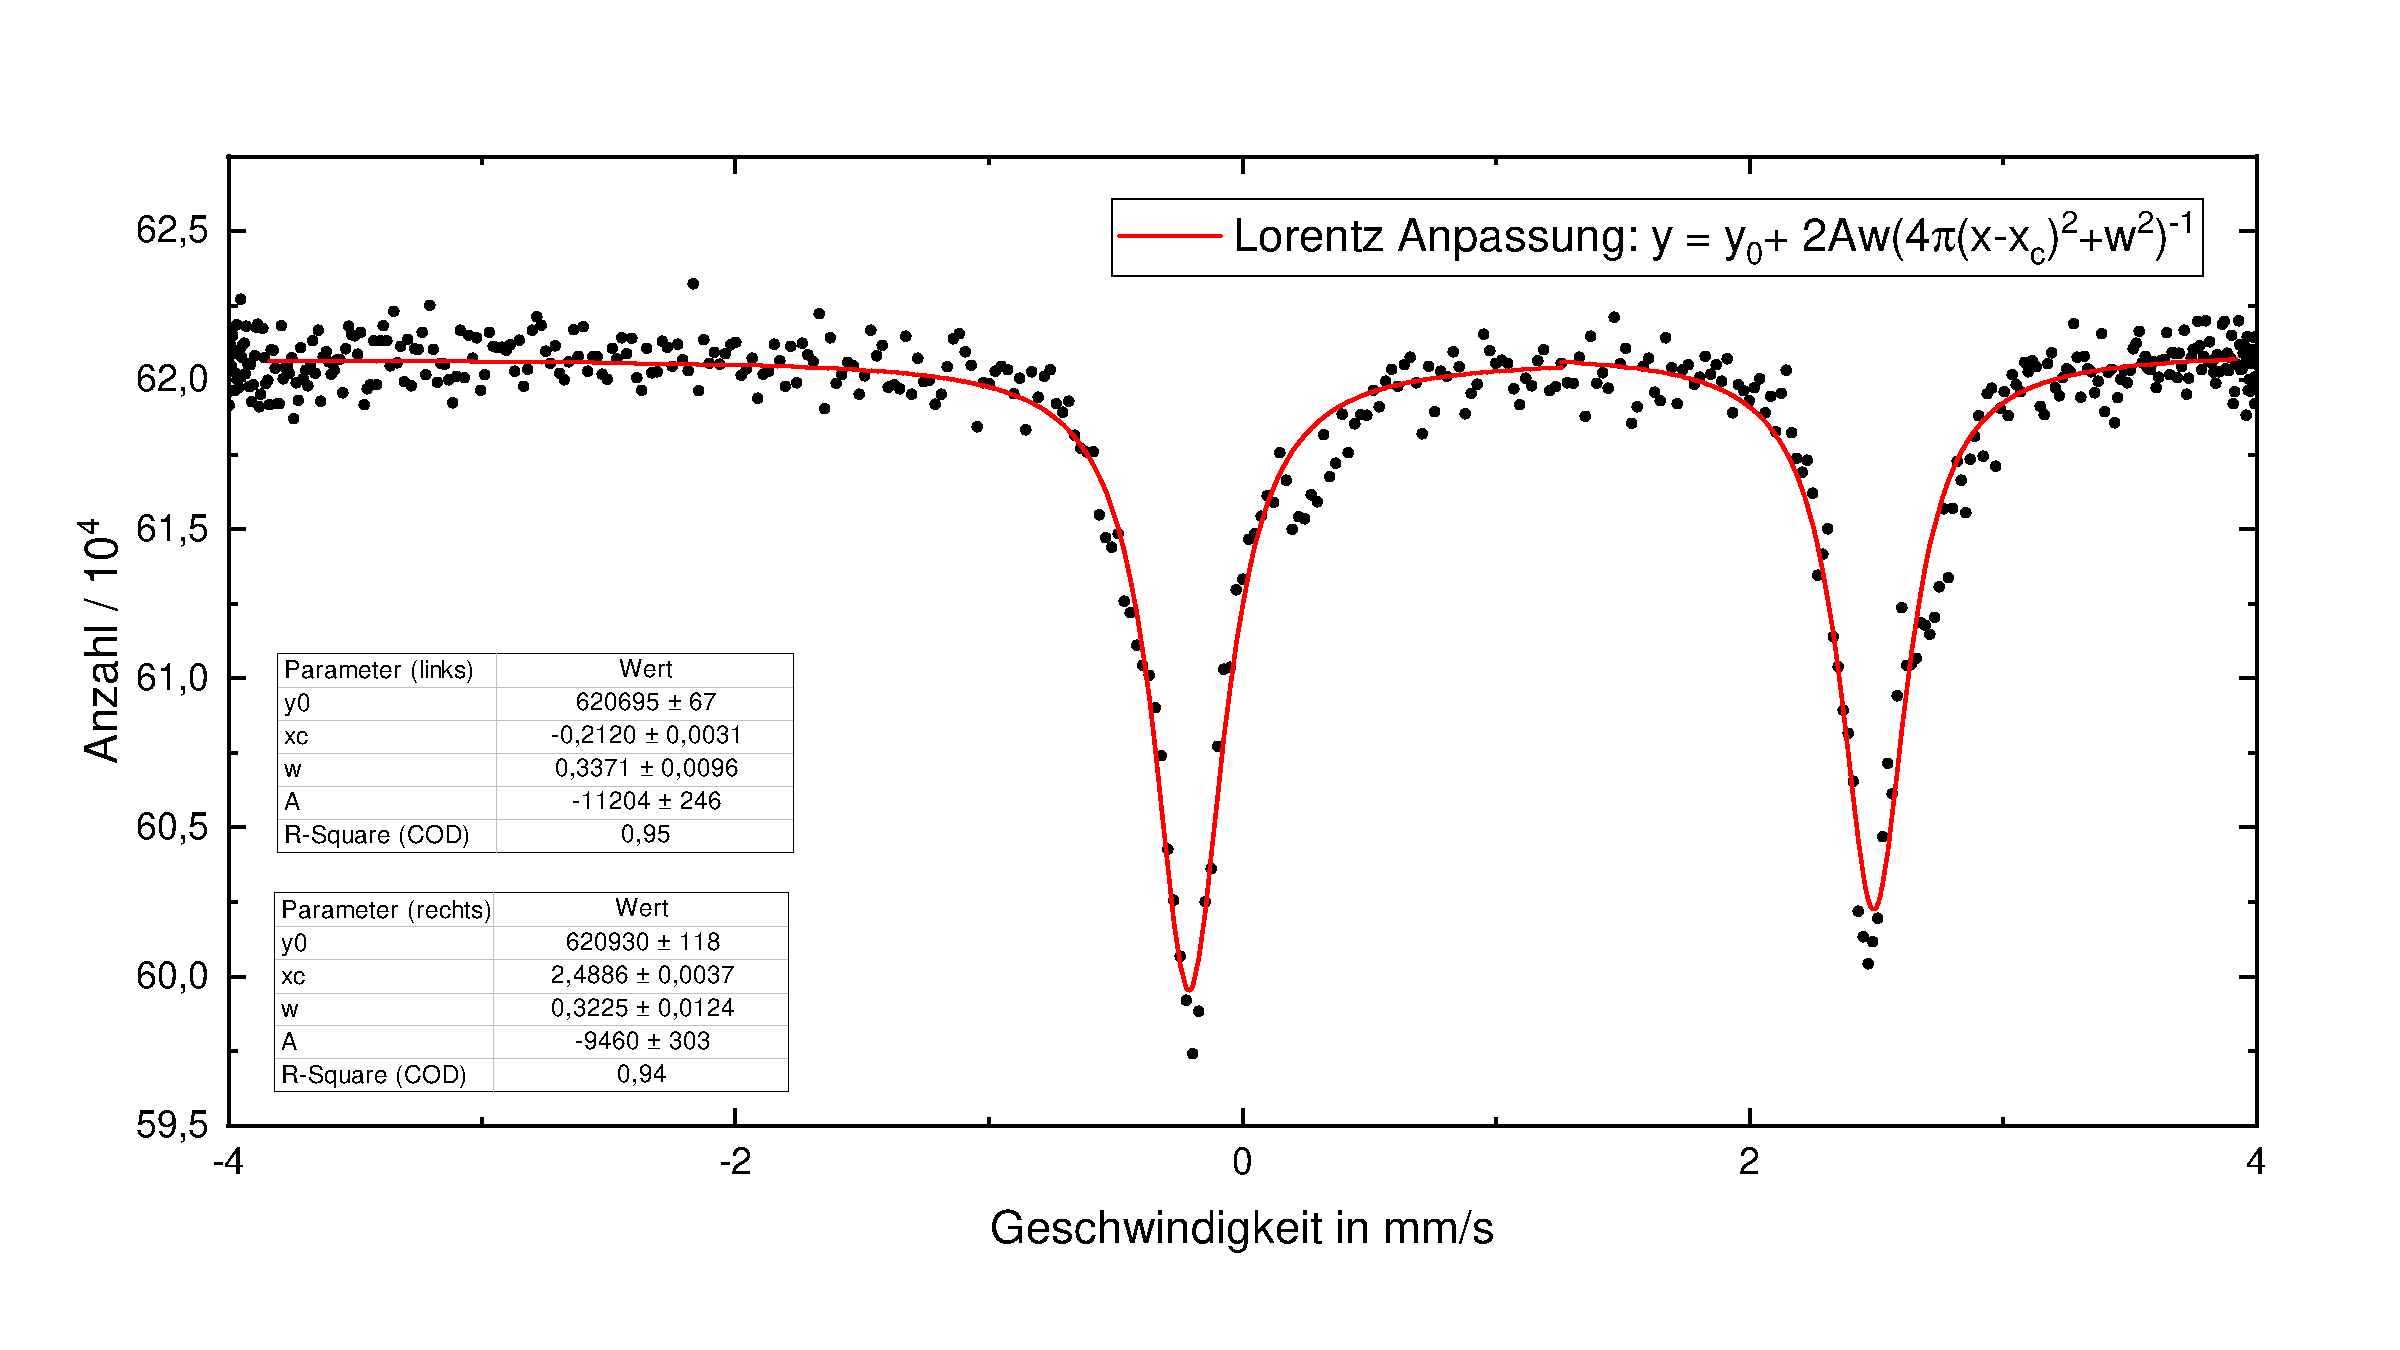
\includegraphics[width=0.95\textwidth]{Bilder/Moessbauer_FeSO4_Lorentz.pdf}
    \caption{Mößbauerspektrum von Eisensulfat (FeSO$_4$). Die Anpassung der Fitfunktion erfolgte durch eine Lorentzanpassung der Form~\eqref{eqn:Lorentzfits}.}
    \label{fig:Moessbauer_FeSO4_Lorentz.pdf}
\end{figure}\\
Die beobachtete Aufspaltung lässt sich auf die elektrische Quadrupolwechselwirkung zurückführen. Im FeSO$_4$ ist das Eisen zweiwertig, die Valenzelektronen sind sechs 3$d$-Elektronen. Die ersten fünf Elektronen führen zu einer halbbesetzten 3$d$-Schale und tragen aufgrund der kugelsymmetrischen Ladungsverteilung nicht zum elektrischen Feldgradienten $V_{zz}$ bei~\cite{Schatz}. Der Feldgradient wird durch das sechste Elektron außerhalb der halbgefüllten 3$d$-Schale bestimmt.\\
Die Quadrupolaufspaltung ergibt sich als Abstand der beiden Absorptionslinien
\begin{align}
  \Delta v = x_{c2} - x_{c1} = \SI[per-mode=fraction, separate-uncertainty]{2,7006 \pm 0,0068}{\milli\metre\per\second}.
\end{align}
Die zugehörige Energieauspaltung ergibt sich nach Gleichung \eqref{eqn:Energieaufspaltung} zu
\begin{align}
  \Delta E_Q = \SI[per-mode=fraction, separate-uncertainty]{129,72
\pm 0,33e-9}{\electronvolt}.
\end{align}
Die Aufspaltung verläuft nicht symmetrisch zum Nullpunkt, da zusätzlich noch eine Isomerieverschiebung vorliegt. Diese ergibt sich wieder als das arithmetische Mittel der beiden Mößbauerlinien und berechnet sich zu
\begin{align}
  v_\text{res} &= \frac{x_{c2} + x_{c1}}{2} = \SI[per-mode=fraction, separate-uncertainty]{1,1383 \pm 0,0068}{\milli\metre\per\second}\\
  E_\text{res} &= \SI[per-mode=fraction, separate-uncertainty]{54,68
\pm 0,33e-9}{\electronvolt}.
\end{align}
Die Linienbreiten lassen sich mithilfe des Fitparameters $w$ gewinnen und sind in Tabelle~\ref{tab:Linienbreite_Eisensulfat} zusammengefasst.
\begin{table}[ht]
	\centering
	\caption{Bestimmung der Linienbreite von Eisensulfat. }
	\label{tab:Linienbreite_Eisensulfat}
  \begin{tabular}{c S[table-format=1.4(5),separate-uncertainty] S[table-format=2.2(3),separate-uncertainty]}
  \toprule
  {Nr.} & {$v_\text{Linie}$ [\si{\milli\metre\per\second}]} & {$E_\text{Linie}$ [\SI{e-9}{\electronvolt}]}\\
   \midrule
   1& 0,3371	\pm 0,0096 & 16,19\pm	0,46\\
   2& 0,3225	\pm0,0124 & 15,49\pm	0,60\\
  \midrule
  \addlinespace
  \textbf{Mittelwert}  & 0,330\pm	0,072 & 15,9	\pm 3,5\\ \bottomrule
  \end{tabular}
\end{table}\\

% *********************************************
% ***** KAPITEL 5 *****************************
% *********************************************
\section{Zusammenfassung}
Die Bedeutung der Mößbauerspektroskopie als wichtiges Analyseverfahren kann im Versuch bestätigt werden. Bei der Untersuchung von Eisen kann dessen Hyperfeinstrukturaufspaltung erkannt, vermessen, und daraus die Energieaufspaltungen des Grundzustands und des angeregten Zustands bestimmt werden. Damit gelingt es, das Magnetfeld am Ort der \textsuperscript{57}Fe Kerne so genau zu berechnen, dass es im Fehlerbereich mit den Literaturwerten übereinstimmt. Außerdem wird auch die Isomerieverschiebung des Eisens bestimmt. Edelstahl als Legierung zeigt keine magnetische Aufspaltung, dafür aber eine effektive Isomerieverschiebung, die sich aus unterschiedlichen dicht beieinander liegenden einzelnen Isomerieverschiebungen ergibt und durch die Mößbauerspektroskopie vermessen werden kann. Mit Eisensulfat wurde ein Stoff untersucht, bei welchem durch die Mößbauerspektroskopie seine elektrische Quadropulaufspaltung beobachtet werden kann. Hierbei kann ebenfalls eine Energieaufspaltung bestimmt werden. \\
Zusammenfassend kann gezeigt werden, dass mit der Mößbauerspektroskopie erfolgreich Isomerieverschiebung, Linienbreite, Hyperfeinstrukturaufspaltungen und Quadropulaufspaltungen vermessen werden können. Darüber hinaus können damit weitere Schlussfolgerungen gezogen und Informationen gewonnen werden. So gelingt es, aus der magnetischen Aufspaltung Magnetfelder am Kern zu bestimmen und aus den Verhältnissen der Absorptionslinien die Richtung des $B$-Feldes zu ermitteln.
% ***** Literaturverzeichnis ******************

\begin{thebibliography}{xxx}
	\bibitem{Schatz}
	G. Schatz: \textit{Nukleare Festkörperphysik}. Teubner Stuttgart 1997 (3. Auflage).
  \bibitem{Mayer}
	T. Mayer-Kuckuk: \textit{Kernphysik}. Teubner Stuttgart 1996 (6. Auflage).
  \bibitem{Bethge}
  K. Bethge: \textit{Kernphysik. Eine Einführung}. Springer Verlag Berlin Heidelberg New York 1996
  \bibitem{Demtroeder}
  W. Demtroeder: \textit{Experimentalphysik 3: Atome, Moleküle und Festkörper}. Springer-Verlag Berlin Heidelberg 2016 (5. Auflage)
	\bibitem{Reisloehner}
  U. Reislöhner: \textit{FSU Fortgeschrittenenen Praktikum: Mößbauer Spektroskopie}, Fried\-rich-Schil\-ler-Uni\-versi\-tät März 2017
  \bibitem{Leifi}
  \url{https://www.leifiphysik.de/sites/default/files/medien/gamma-spektrum-cs137.svg}, Stand: 03.01.2020
  % \bibitem{Grossberger}
  % \url{http://www.grossberger.net/atomphysik/gamma1.html}, Stand: 03.01.2020
\end{thebibliography}

\end{document}
